\documentclass[12pt]{article}
\usepackage{amsmath,amssymb,amsthm}
\usepackage{geometry}
\usepackage{graphicx}
\usepackage{cite}
\usepackage{float}

\title{Report 3: Generalized Malaria Transmission Model with Arbitrary Erlang-Distributed Latent Stages}
\author{Yaghoub Shahmari}
\date{\today}

\begin{document}
\maketitle

\begin{abstract}
This report presents a generalized malaria transmission model extending the Ross-Macdonald framework by incorporating an arbitrary number of latent compartments for both treated and untreated mosquito populations, with transitions governed by Erlang distributions. The model explicitly tracks human and mosquito compartments, accounting for treatment coupling and sequential progression through latent stages. We formulate the corresponding system of ordinary differential equations (ODEs), derive the structure of the Next Generation Matrix (NGM) for computing the basic reproduction number \(R_0\), and outline methods for determining both analytical and numerical endemic equilibria. This framework provides a flexible platform to explore the impact of latent period distributions on malaria dynamics.
\end{abstract}

\section{Introduction}

Classical malaria transmission models typically adopt a Ross-Macdonald structure with a fixed number of latent stages in mosquito populations, often assuming exponential or Erlang-distributed latent periods via two compartments. To generalize this framework and better capture variability in mosquito latency, we extend the model to support arbitrary numbers of latent stages in both treated and untreated mosquito subpopulations. The per-stage progression rates are adjusted accordingly so that the total latency duration follows an Erlang distribution with a fixed mean.

This generalization allows investigation into how the shape of the latent period distribution affects key epidemiological quantities such as the basic reproduction number \(R_0\) and the endemic equilibrium.

\section{Model Structure and Dynamics}

\subsection{Compartments and Notation}

The model divides the host and mosquito populations into the following compartments:
\begin{itemize}
    \item \textbf{Humans:}
    \[
    S_H \text{ (susceptible)}, \quad I_H \text{ (infected)}.
    \]
    \item \textbf{Untreated Mosquitoes:}
    \[
    S_M,\, E_{1,M},\, E_{2,M},\, \dots,\, E_{L_{NM},M},\, I_M.
    \]
    \item \textbf{Treated Mosquitoes:}
    \[
    S_T,\, E_{1,T},\, E_{2,T},\, \dots,\, E_{L_{NT},T},\, I_T.
    \]
\end{itemize}
The numbers \(L_{NM}\) and \(L_{NT}\) represent the number of latent stages for untreated and treated mosquitoes, respectively.

\subsection{Disease-Free Equilibrium (DFE)}

At the DFE, \(I_H = 0\) and all infected mosquito compartments are zero. The susceptible mosquito compartments are determined by solving:
\[
\begin{pmatrix}
-(t + g) & h \\
t & -(h+g)
\end{pmatrix}
\begin{pmatrix}
S_M^* \\ S_T^*
\end{pmatrix}
=
\begin{pmatrix}
-g \\ 0
\end{pmatrix}
\]
yielding the equilibrium values \(S_M^*\) and \(S_T^*\).

\subsection{Generalized ODE System}

The dynamics are governed by the following ODEs:

\paragraph{Humans (SIS):}
\begin{align*}
\frac{dS_H}{dt} &= -m a b (I_M + I_T) S_H + r I_H, \\
\frac{dI_H}{dt} &= m a b (I_M + I_T) S_H - r I_H.
\end{align*}

\paragraph{Untreated Mosquitoes:}
\begin{align*}
\frac{dS_M}{dt} &= g + h S_T - a c I_H S_M - t S_M - g S_M, \\
\frac{dE_{1,M}}{dt} &= a c I_H S_M - (t + s_M/L_{NM} + g) E_{1,M}, \\
\frac{dE_{i,M}}{dt} &= \frac{s_M}{L_{NM}} E_{i-1,M} - \left(\frac{s_M}{L_{NM}} + g \right) E_{i,M}, \quad i=2,\dots,L_{NM}, \\
\frac{dI_M}{dt} &= \frac{s_M}{L_{NM}} E_{L_{NM},M} - g I_M.
\end{align*}

\paragraph{Treated Mosquitoes:}
\begin{align*}
\frac{dS_T}{dt} &= t S_M - a c I_H S_T - h S_T - g S_T, \\
\frac{dE_{1,T}}{dt} &= a c I_H S_T + t E_{1,M} - \left(\frac{s_T}{L_{NT}} + g\right) E_{1,T}, \\
\frac{dE_{i,T}}{dt} &= \frac{s_T}{L_{NT}} E_{i-1,T} - \left(\frac{s_T}{L_{NT}} + g \right) E_{i,T}, \quad i=2,\dots,L_{NT}, \\
\frac{dI_T}{dt} &= \frac{s_T}{L_{NT}} E_{L_{NT},T} - g I_T.
\end{align*}

\section{Basic Reproduction Number \(\mathbf{R_0}\)}

The Next Generation Matrix (NGM) method is used to compute \(R_0\). The infected state vector is:
\[
\mathbf{x} = \begin{bmatrix}
I_H,\, E_{1,M},\, \dots,\, E_{L_{NM},M},\, I_M,\, E_{1,T},\, \dots,\, E_{L_{NT},T},\, I_T
\end{bmatrix}^\top.
\]

\subsection{F and V Matrices}

The matrices \(\mathbf{F}\) and \(\mathbf{V}\) represent new infections and transitions respectively.

New infections arise via:
\begin{itemize}
    \item From mosquitoes to humans.
    \item From humans to mosquitoes (first latent stage).
\end{itemize}

Transitions (in \(\mathbf{V}\)) include:
\begin{itemize}
    \item Recovery, death, progression through latent stages, treatment transfer, etc.
\end{itemize}

The NGM is:
\[
\mathbf{NGM} = \mathbf{F} \mathbf{V}^{-1}
\]
and
\[
R_0 = \rho(\mathbf{NGM}),
\]
where \(\rho\) is the spectral radius.

\section{Endemic Equilibrium Calculation}

\subsection{Analytical Approximation}

We derive closed-form expressions for mosquito compartments at endemic equilibrium as functions of \(I_H\), then numerically solve a consistency equation:
\[
\frac{I_H}{1-I_H} = \frac{m a b (I_M(I_H) + I_T(I_H))}{r}
\]
to find \(I_H^*\). The other equilibrium values follow directly.

\subsection{Numerical ODE Integration}

An alternative numerical approach perturbs the DFE by seeding a small infection and iteratively integrates the ODE system. Convergence is assessed by fitting a linear regression to the last \(N\) solution values for each state variable and halting when all slopes fall below a tolerance.

\section{Results}

\subsection{R0 for treatment rate/period parameters}

\begin{figure}[H]
    \centering
    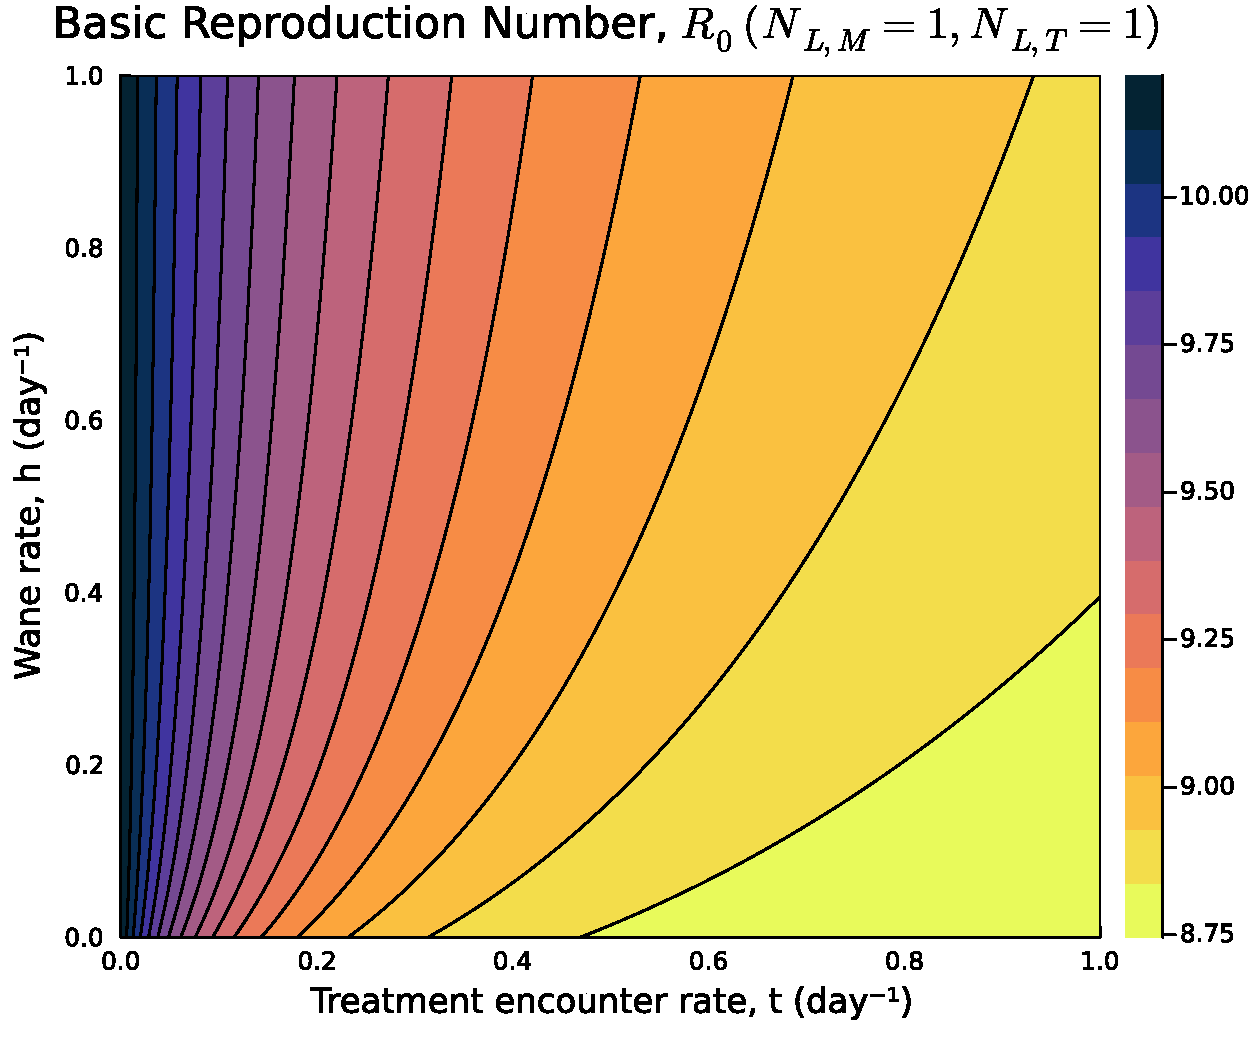
\includegraphics[width=0.4\textwidth]{../../fig/gen_model/R0_rates_txh_1x1.pdf}
    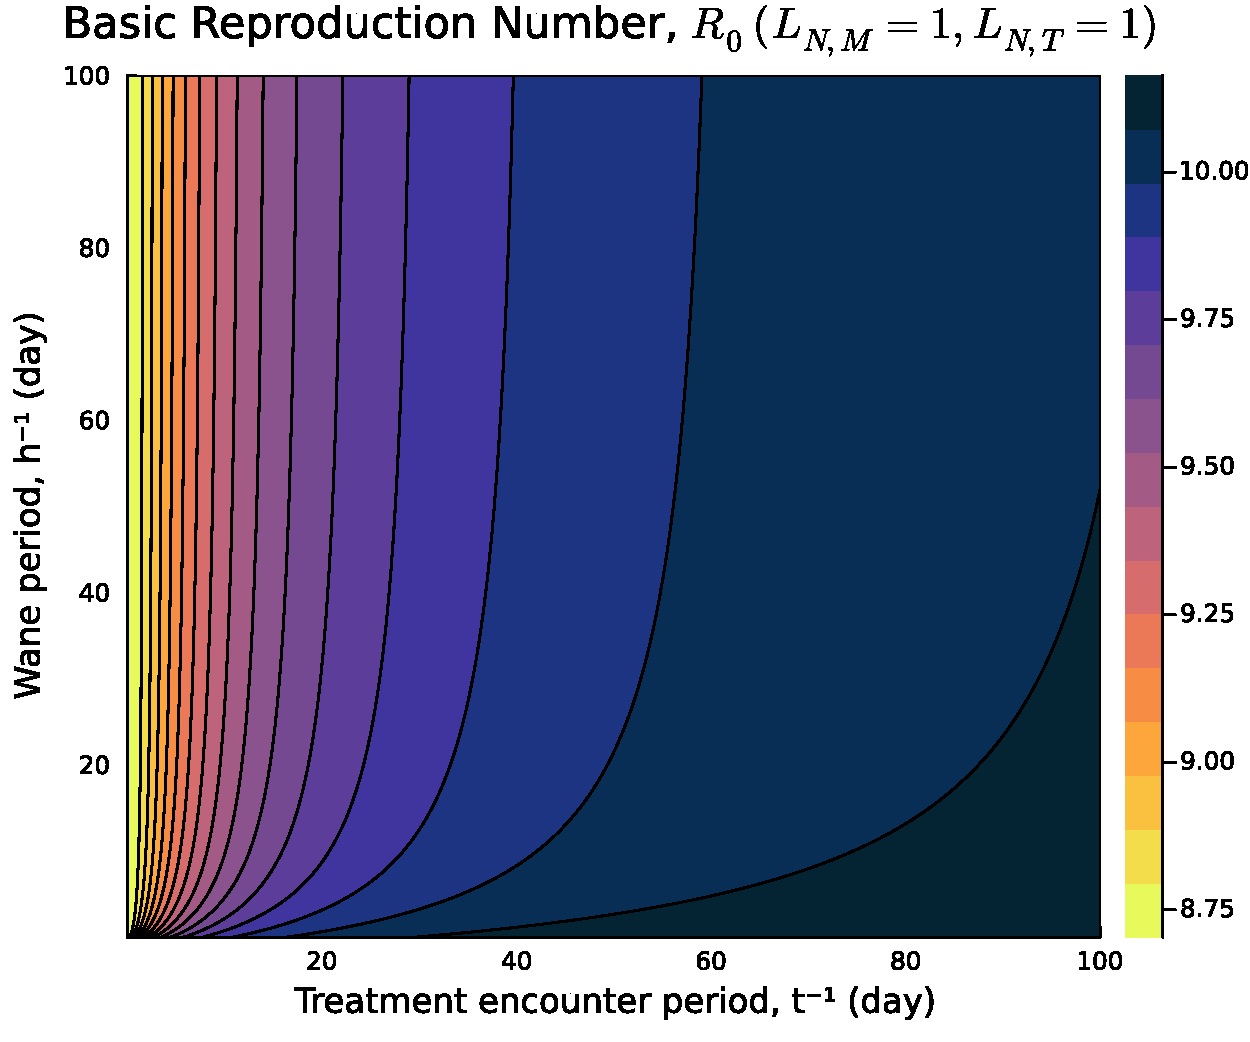
\includegraphics[width=0.4\textwidth]{../../fig/gen_model/R0_periods_txh_1x1.pdf}\\
    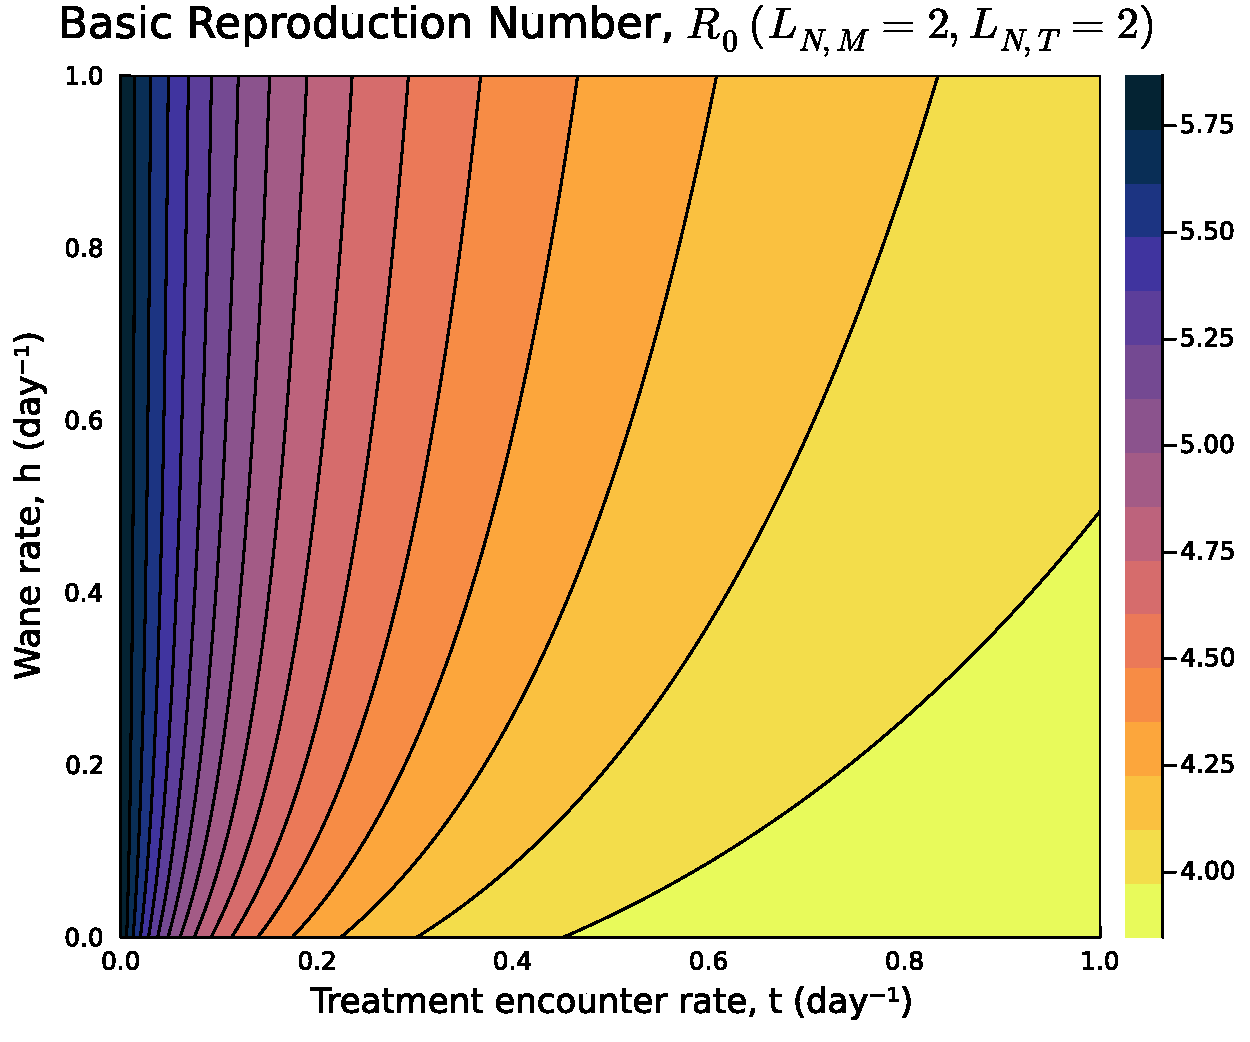
\includegraphics[width=0.4\textwidth]{../../fig/gen_model/R0_rates_txh_2x2.pdf}
    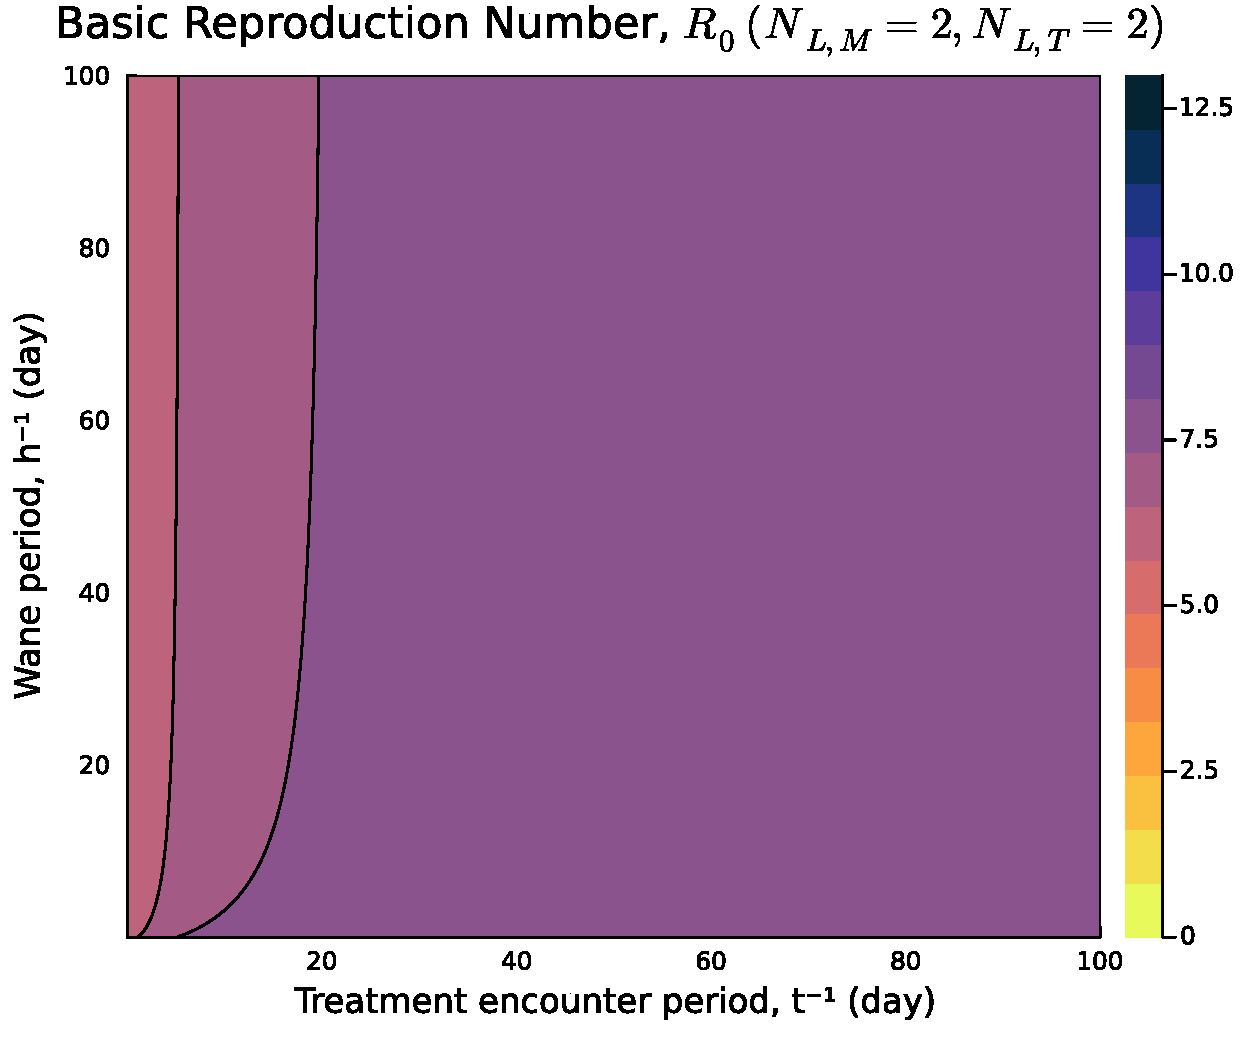
\includegraphics[width=0.4\textwidth]{../../fig/gen_model/R0_periods_txh_2x2.pdf}\\
    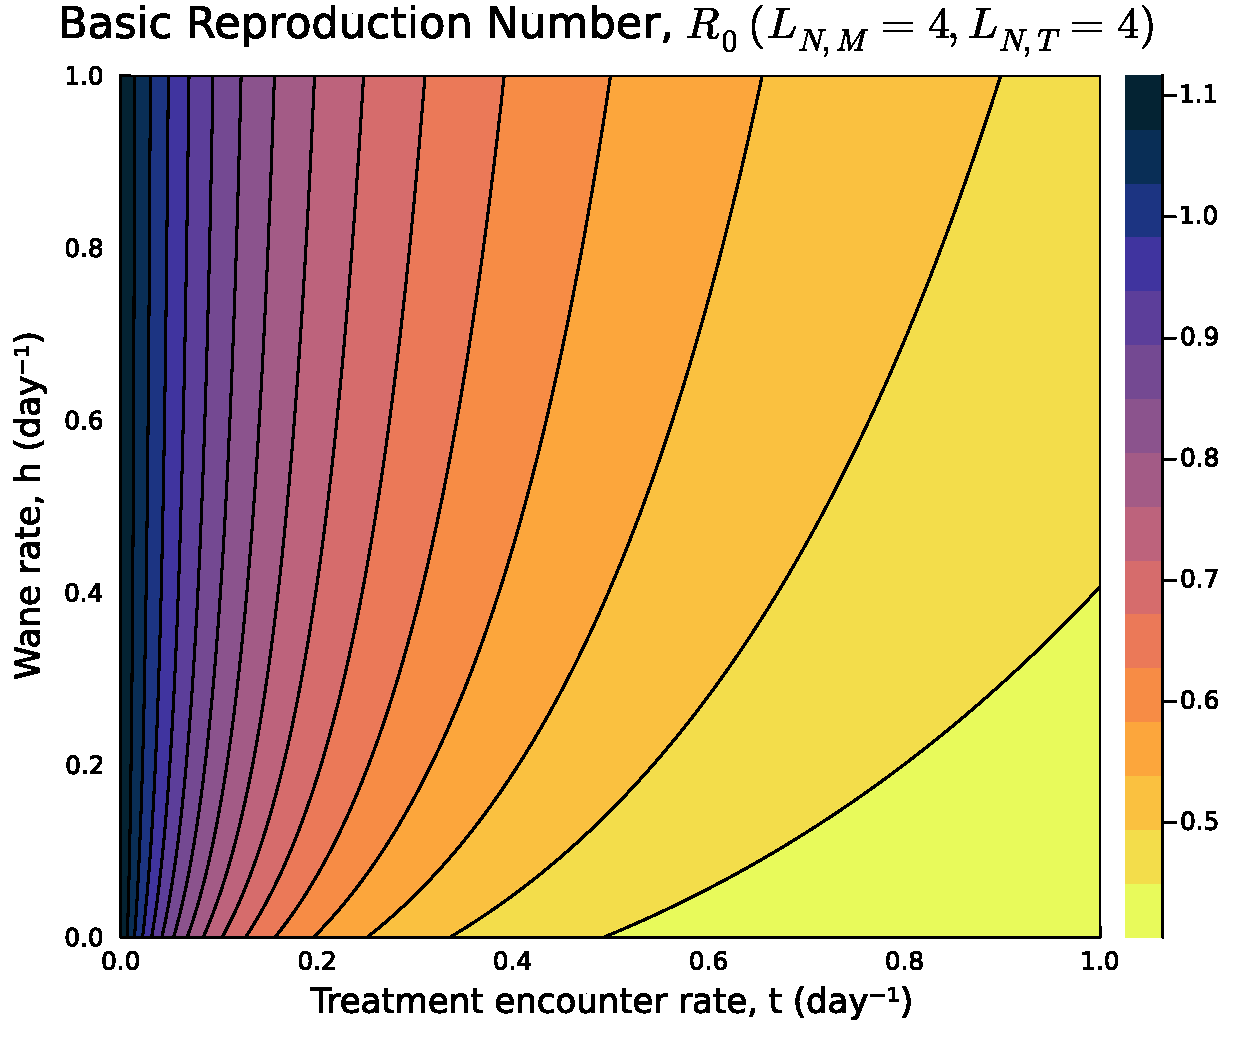
\includegraphics[width=0.4\textwidth]{../../fig/gen_model/R0_rates_txh_4x4.pdf}
    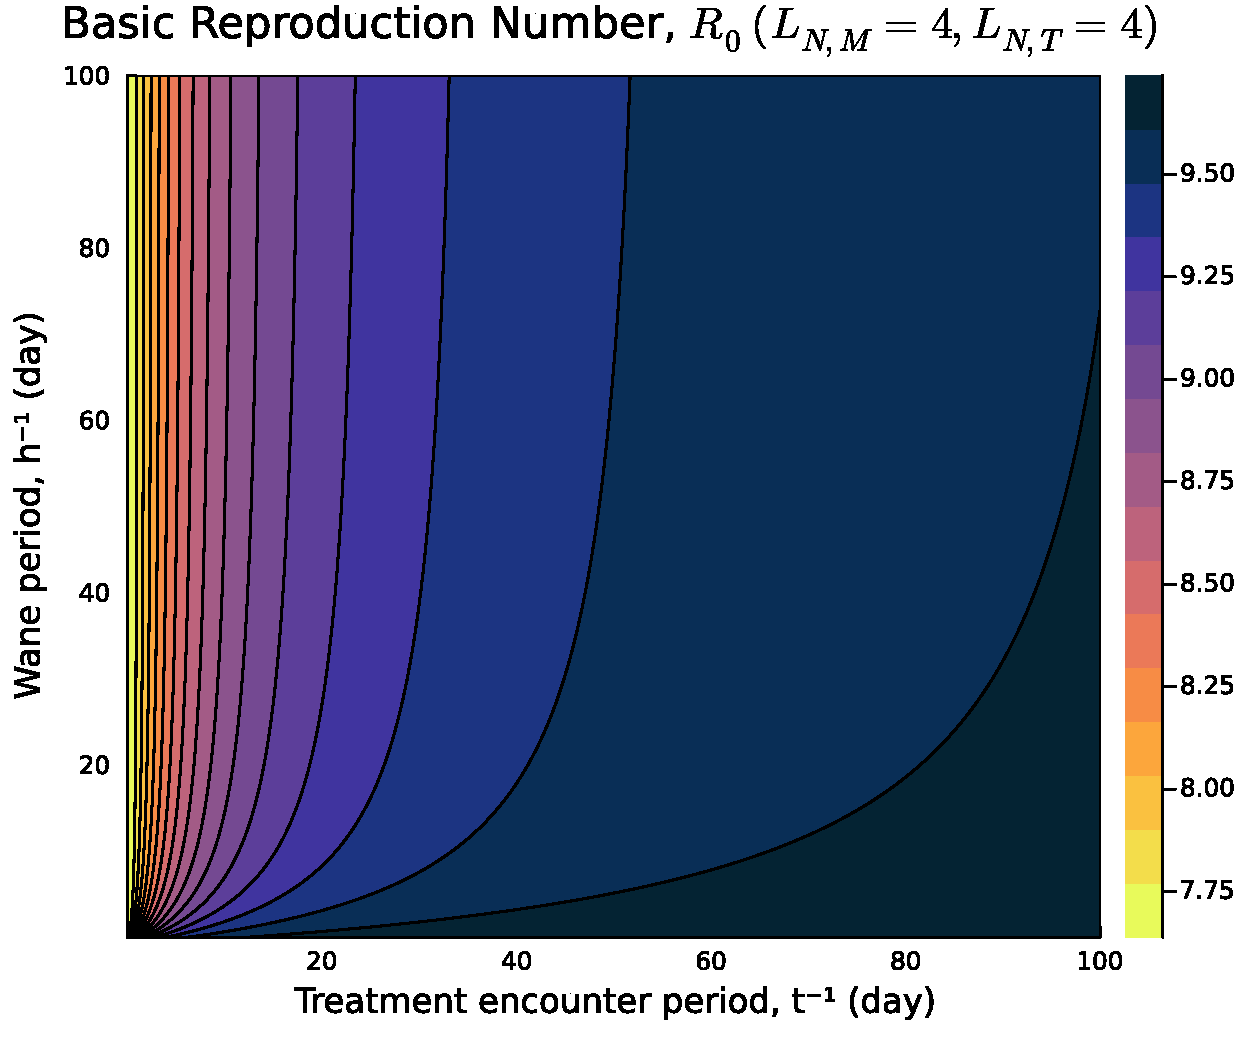
\includegraphics[width=0.4\textwidth]{../../fig/gen_model/R0_periods_txh_4x4.pdf}
    \caption{\textbf{R0 for treatment rate/period parameters.} The left panels show the basic reproduction number \(R_0\) as a function of the treatment rate, while the right panels show \(R_0\) as a function of the treatment period.}
\end{figure}

\begin{figure}[H]
    \centering
    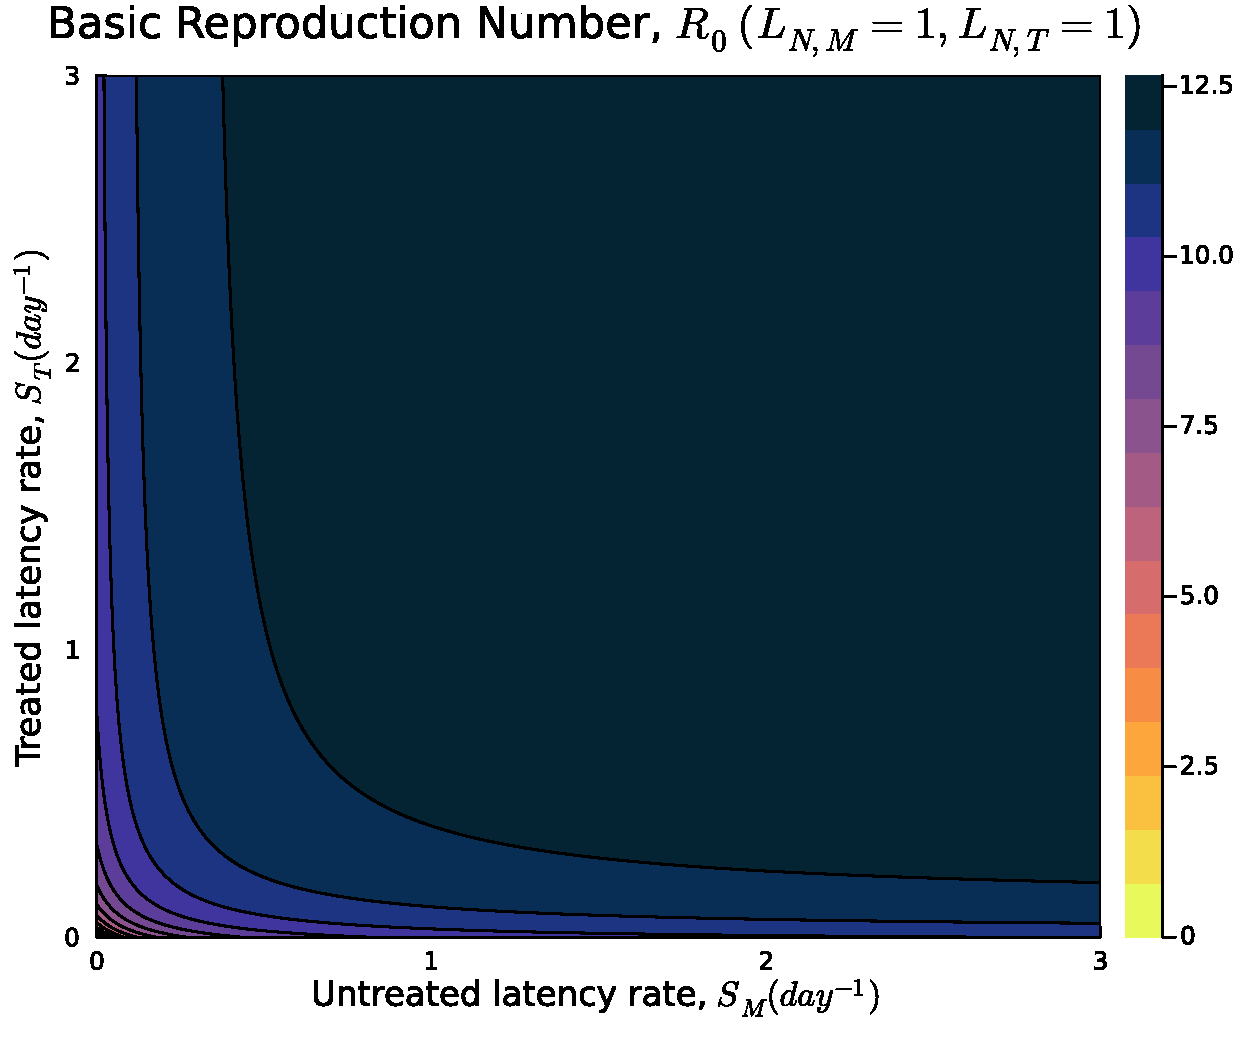
\includegraphics[width=0.4\textwidth]{../../fig/gen_model/R0_rates_SMxST_1x1.pdf}
    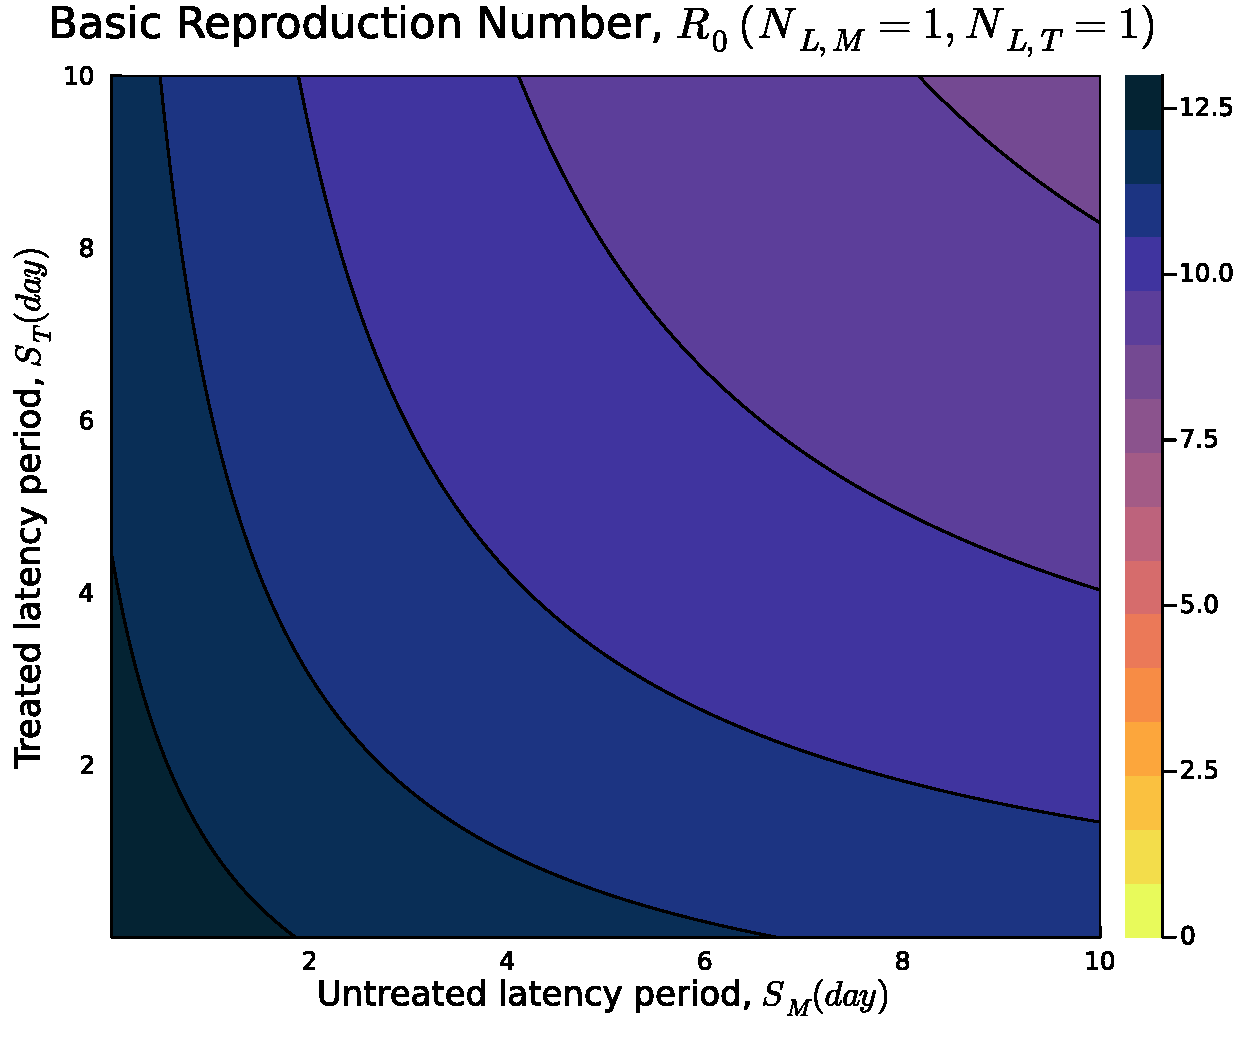
\includegraphics[width=0.4\textwidth]{../../fig/gen_model/R0_periods_SMxST_1x1.pdf}\\
    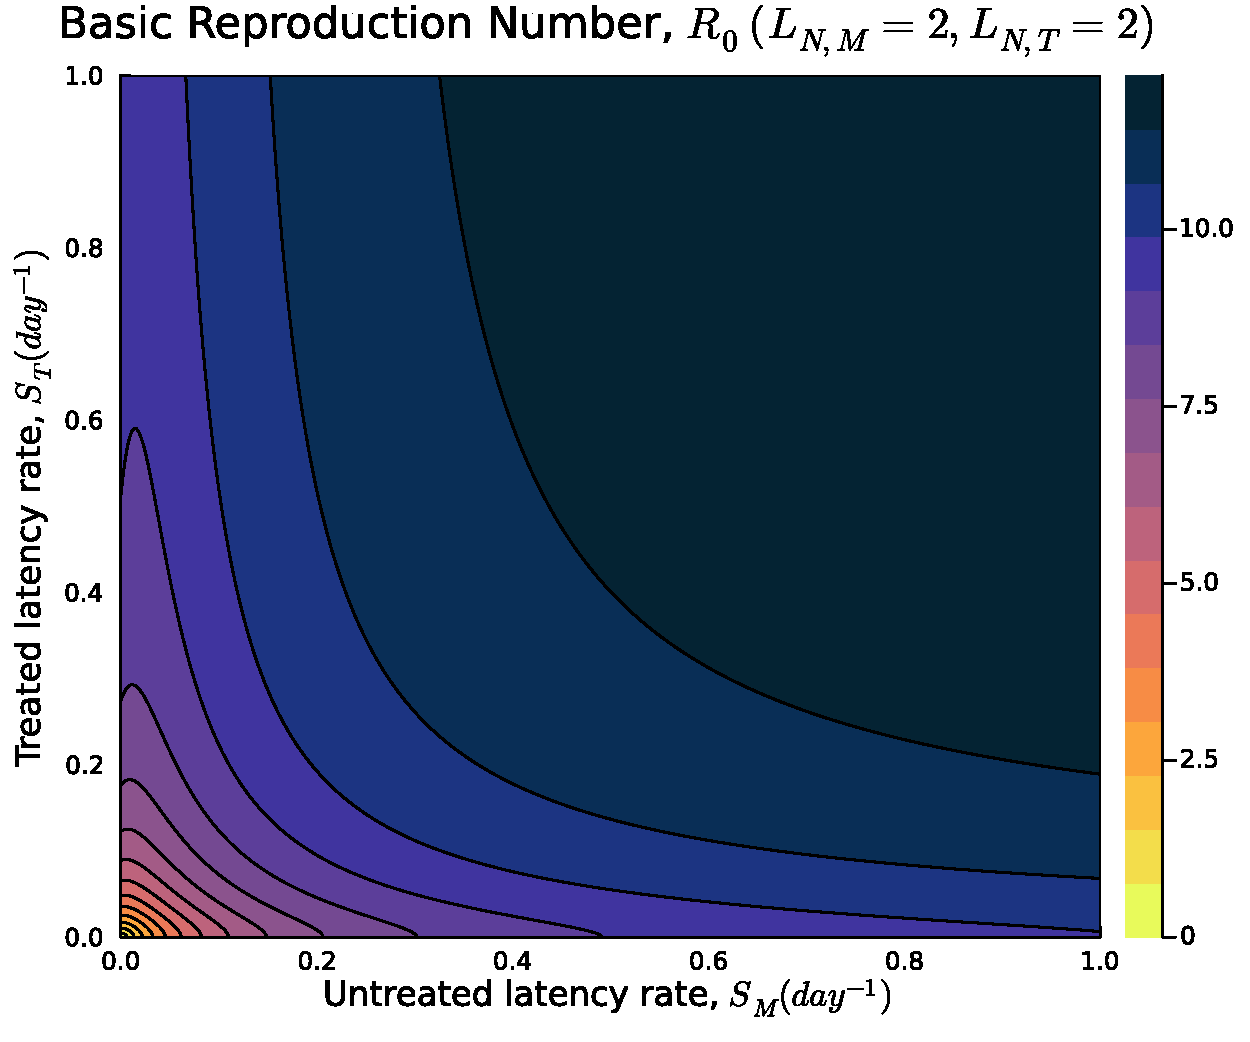
\includegraphics[width=0.4\textwidth]{../../fig/gen_model/R0_rates_SMxST_2x2.pdf}
    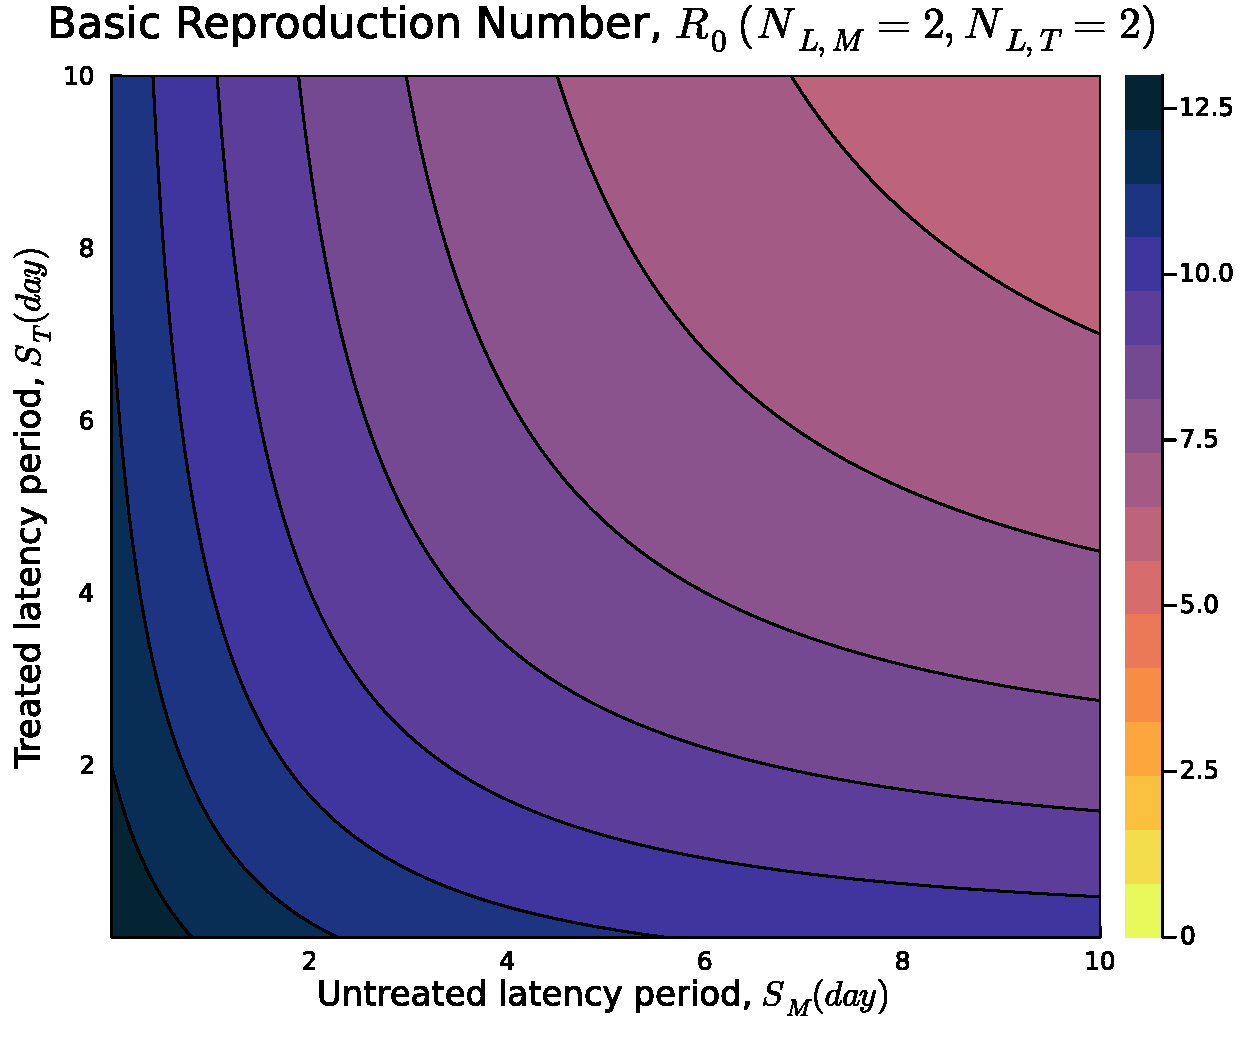
\includegraphics[width=0.4\textwidth]{../../fig/gen_model/R0_periods_SMxST_2x2.pdf}\\
    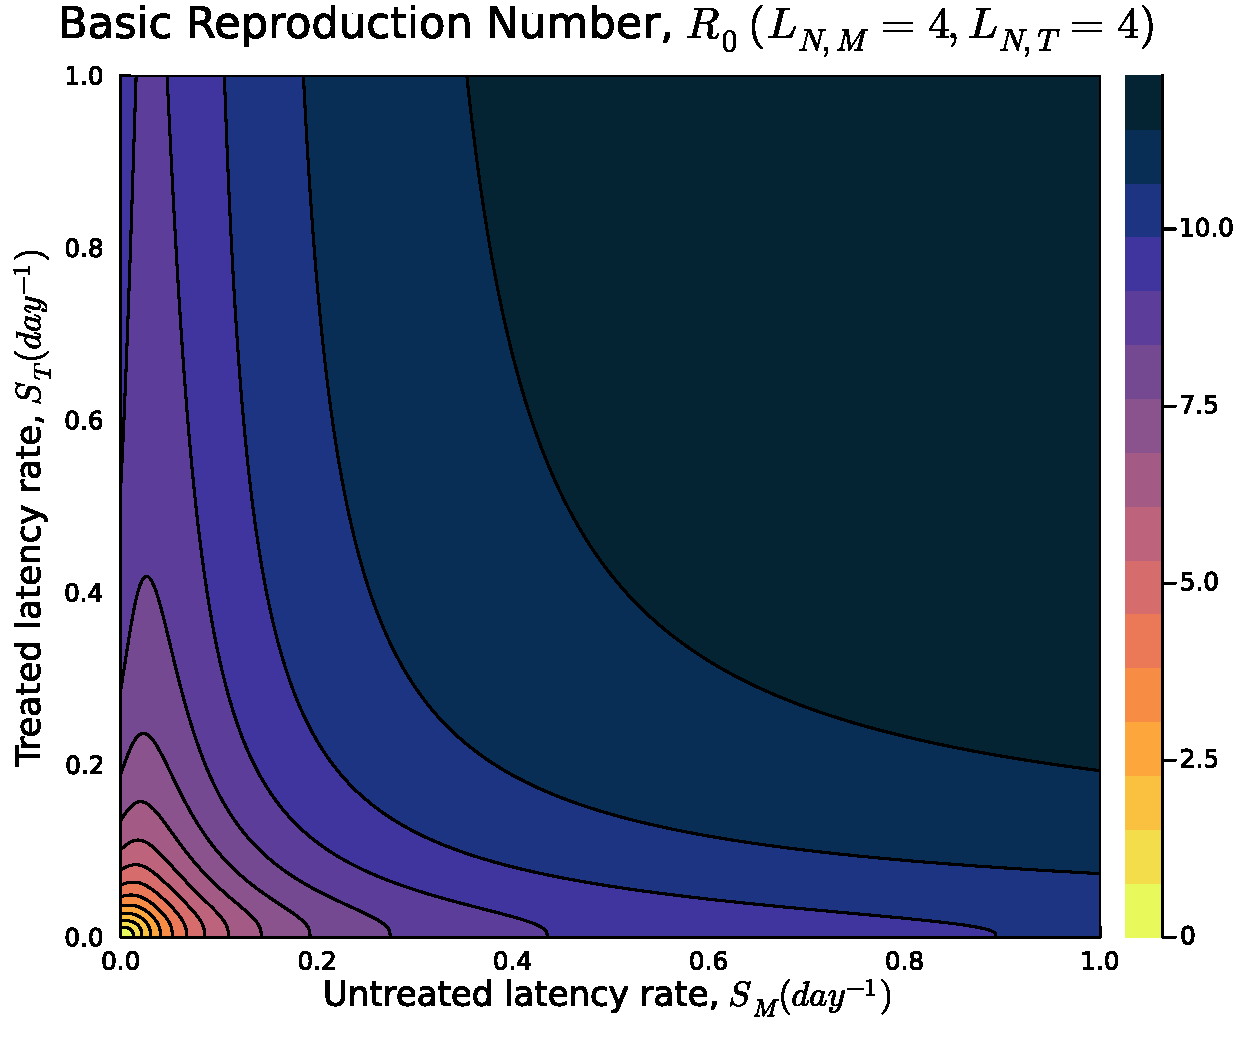
\includegraphics[width=0.4\textwidth]{../../fig/gen_model/R0_rates_SMxST_4x4.pdf}
    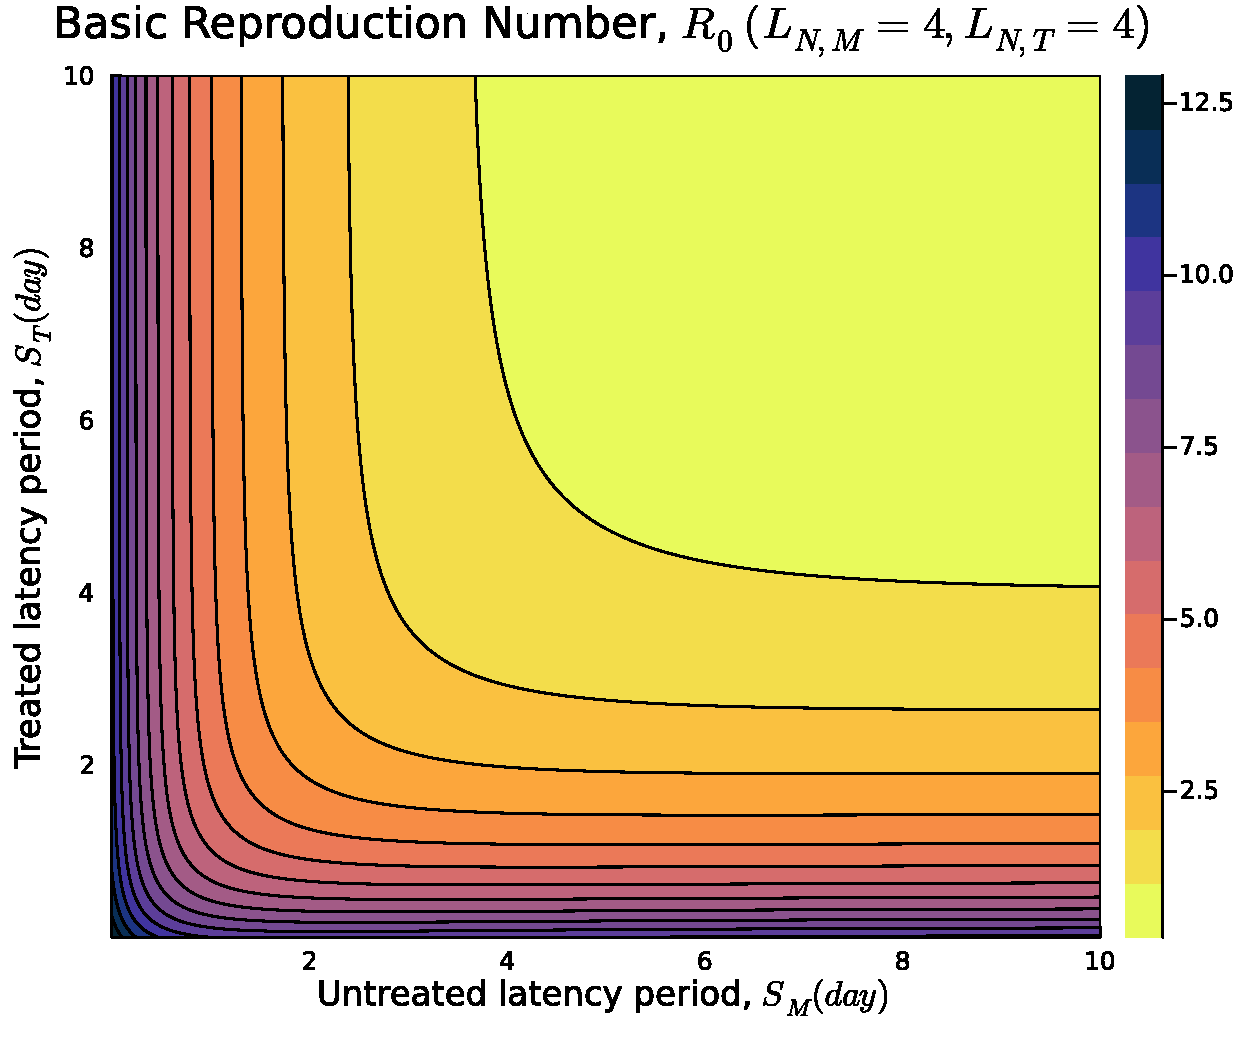
\includegraphics[width=0.4\textwidth]{../../fig/gen_model/R0_periods_SMxST_4x4.pdf}
    \caption{\textbf{R0 for latency rate/period parameters.} The left panels show the basic reproduction number \(R_0\) as a function of the latency rate, while the right panels show \(R_0\) as a function of the latency period.}
\end{figure}

\begin{figure}[H]
    \centering
    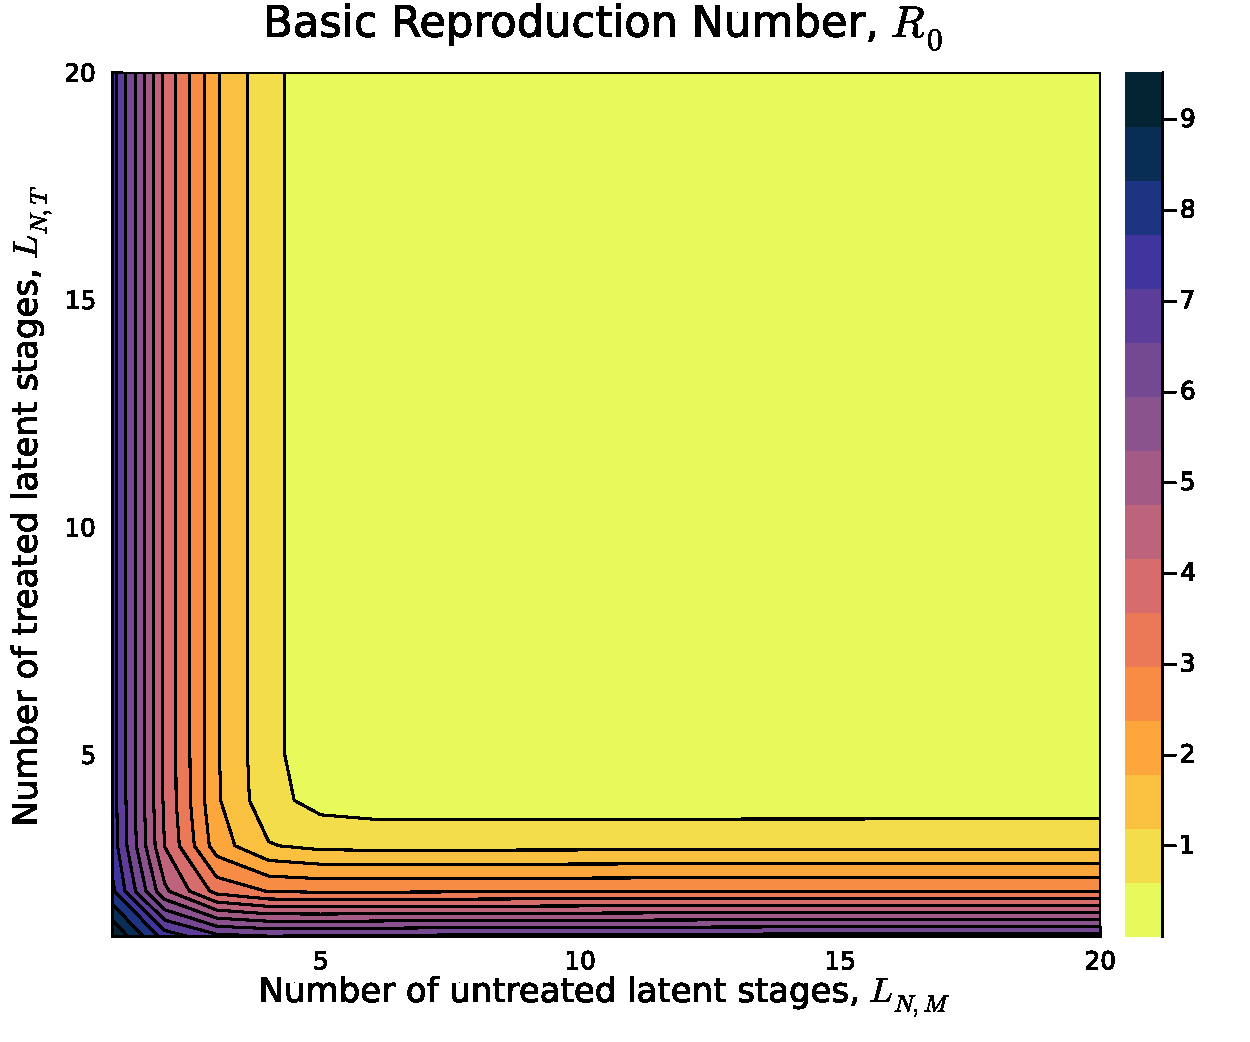
\includegraphics[width=0.4\textwidth]{../../fig/gen_model/R0_NLMxNLT.pdf}
    \caption{\textbf{R0 for number of latent stages.} The basic reproduction number \(R_0\) as a function of the number of latent stages in untreated and treated mosquitoes.}
\end{figure}

\subsection{Infections Humans at endemic equilibrium}

\begin{figure}[H]
    \centering
    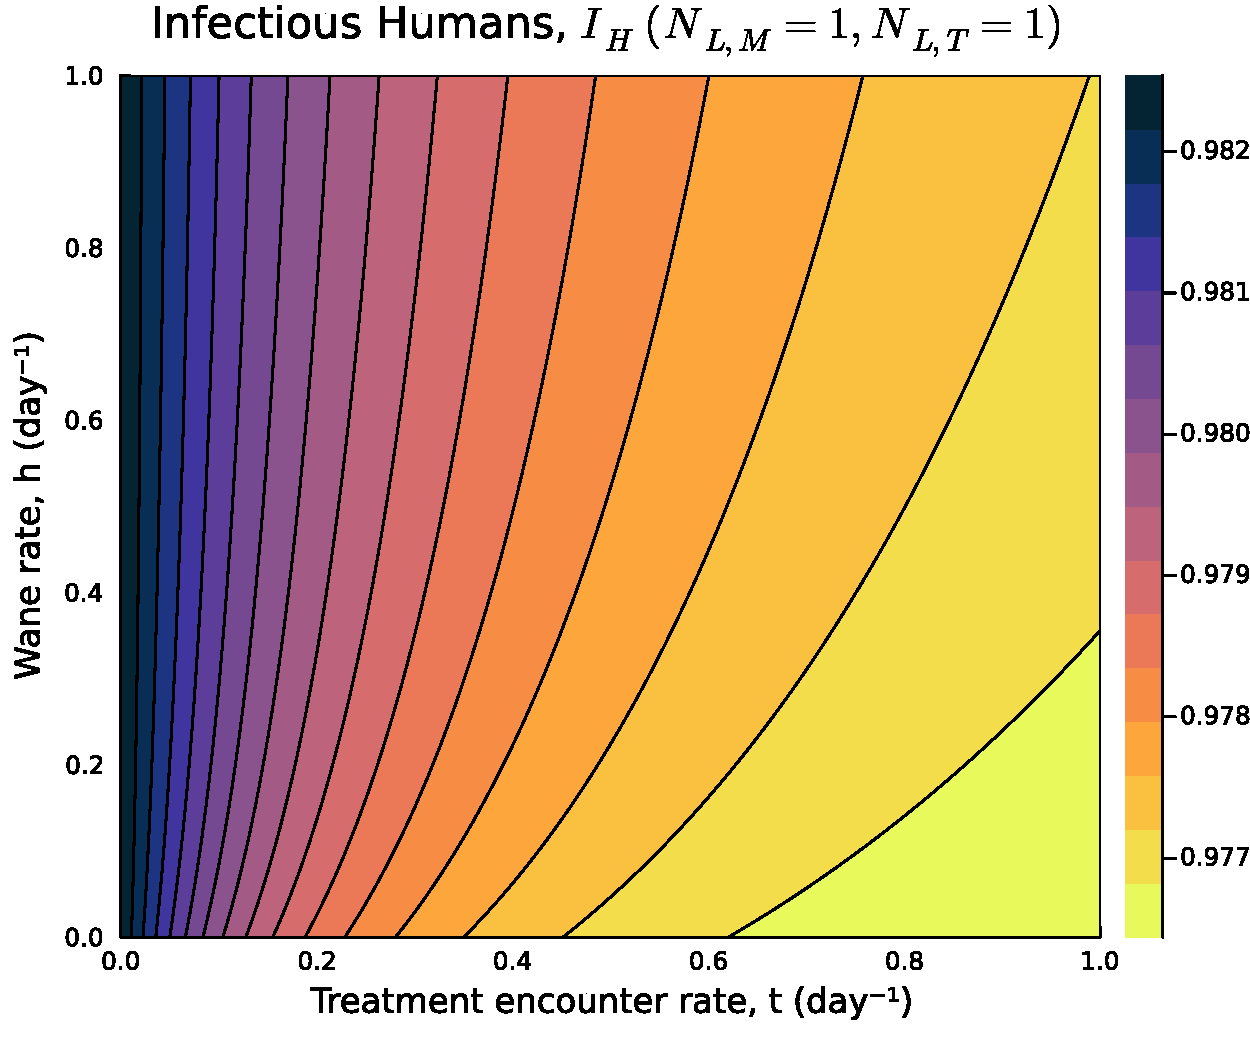
\includegraphics[width=0.4\textwidth]{../../fig/gen_model/IH_rates_txh_1x1.pdf}
    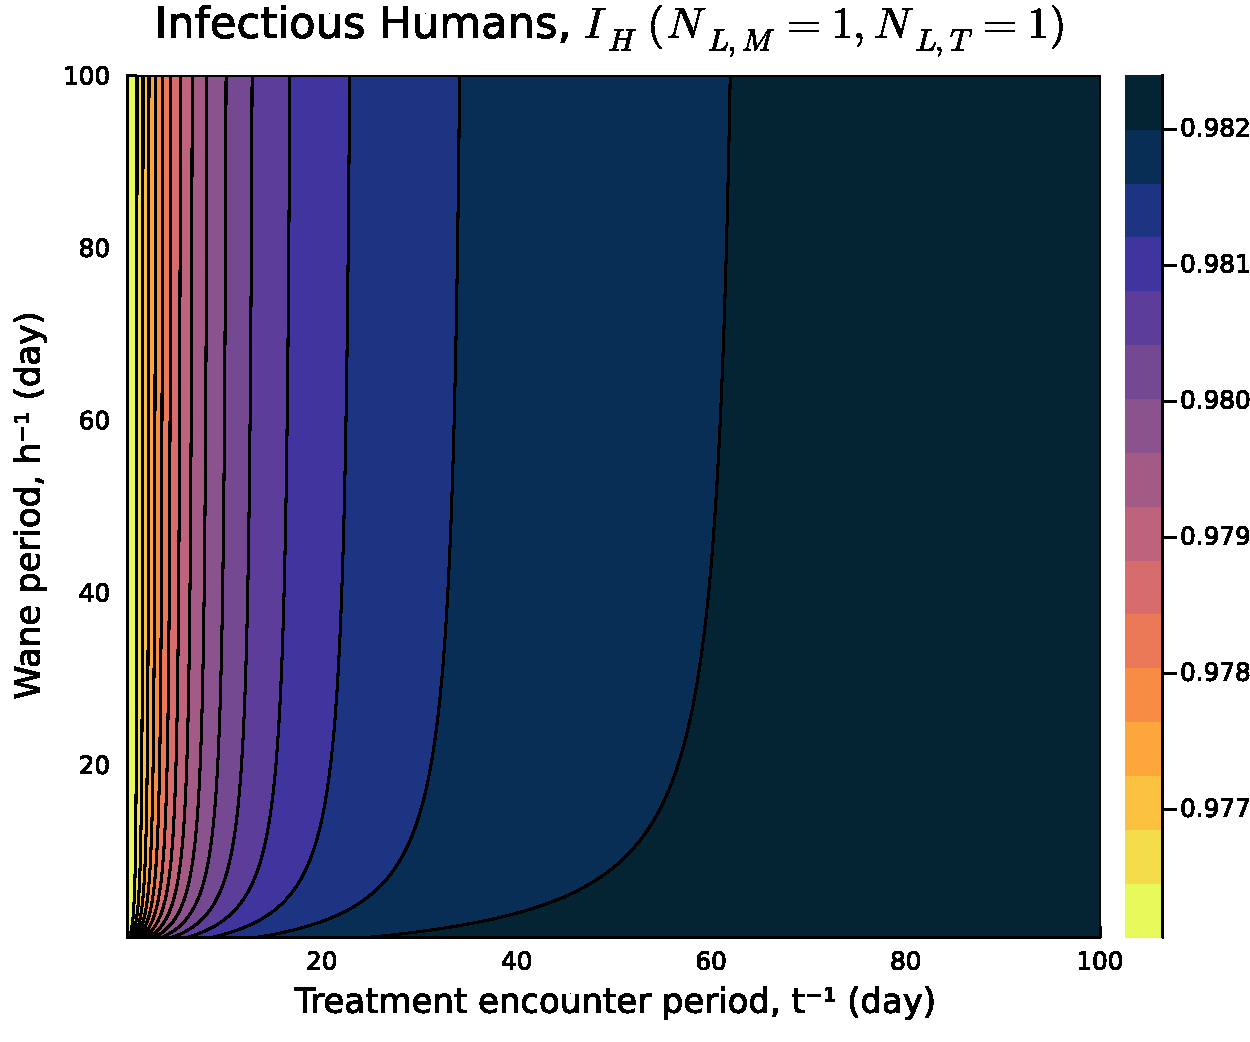
\includegraphics[width=0.4\textwidth]{../../fig/gen_model/IH_periods_txh_1x1.pdf}\\
    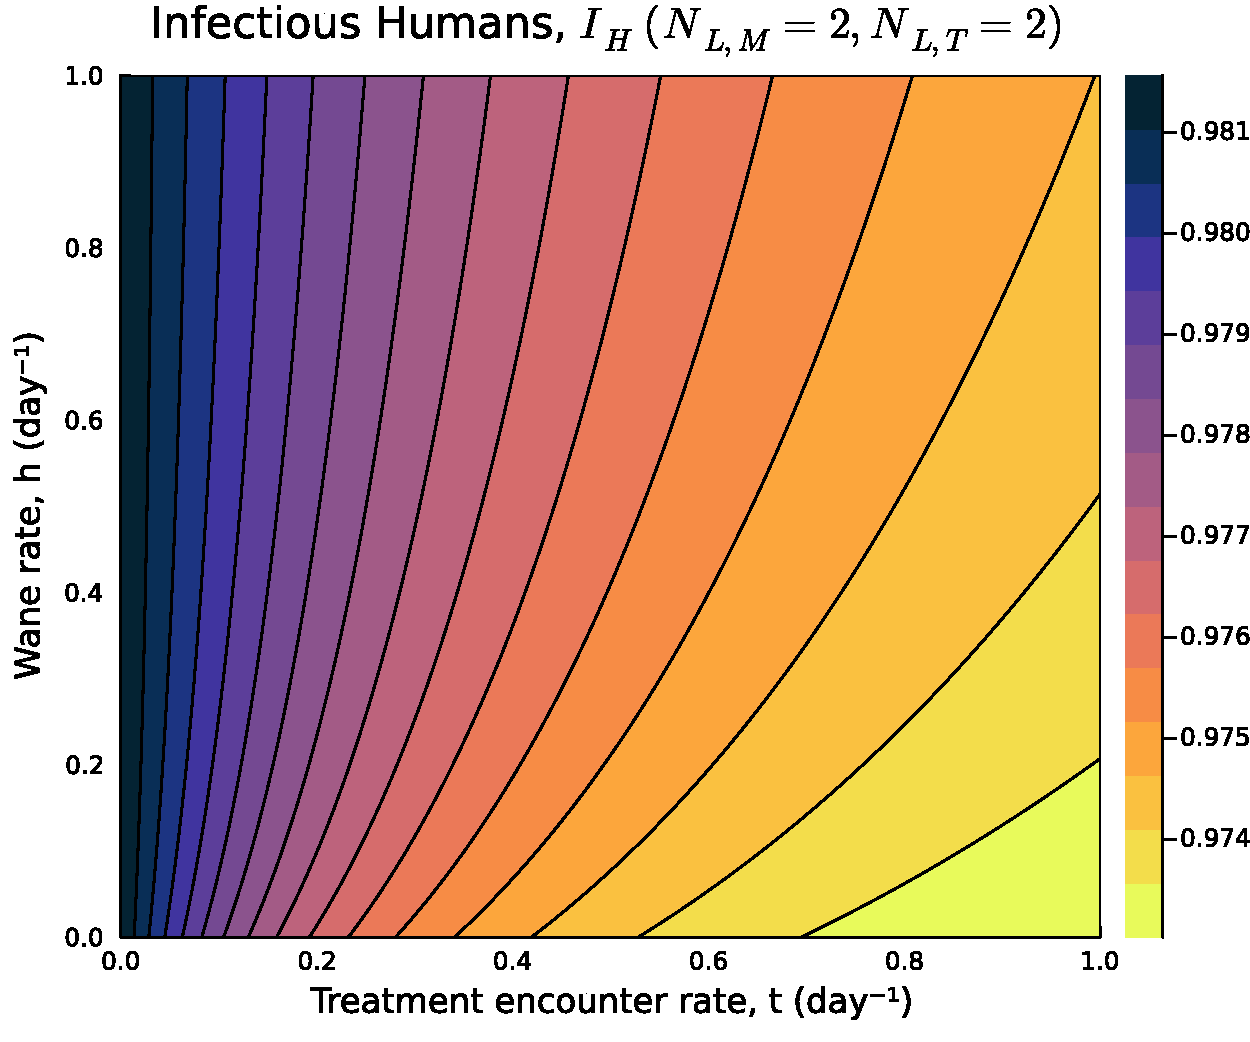
\includegraphics[width=0.4\textwidth]{../../fig/gen_model/IH_rates_txh_2x2.pdf}
    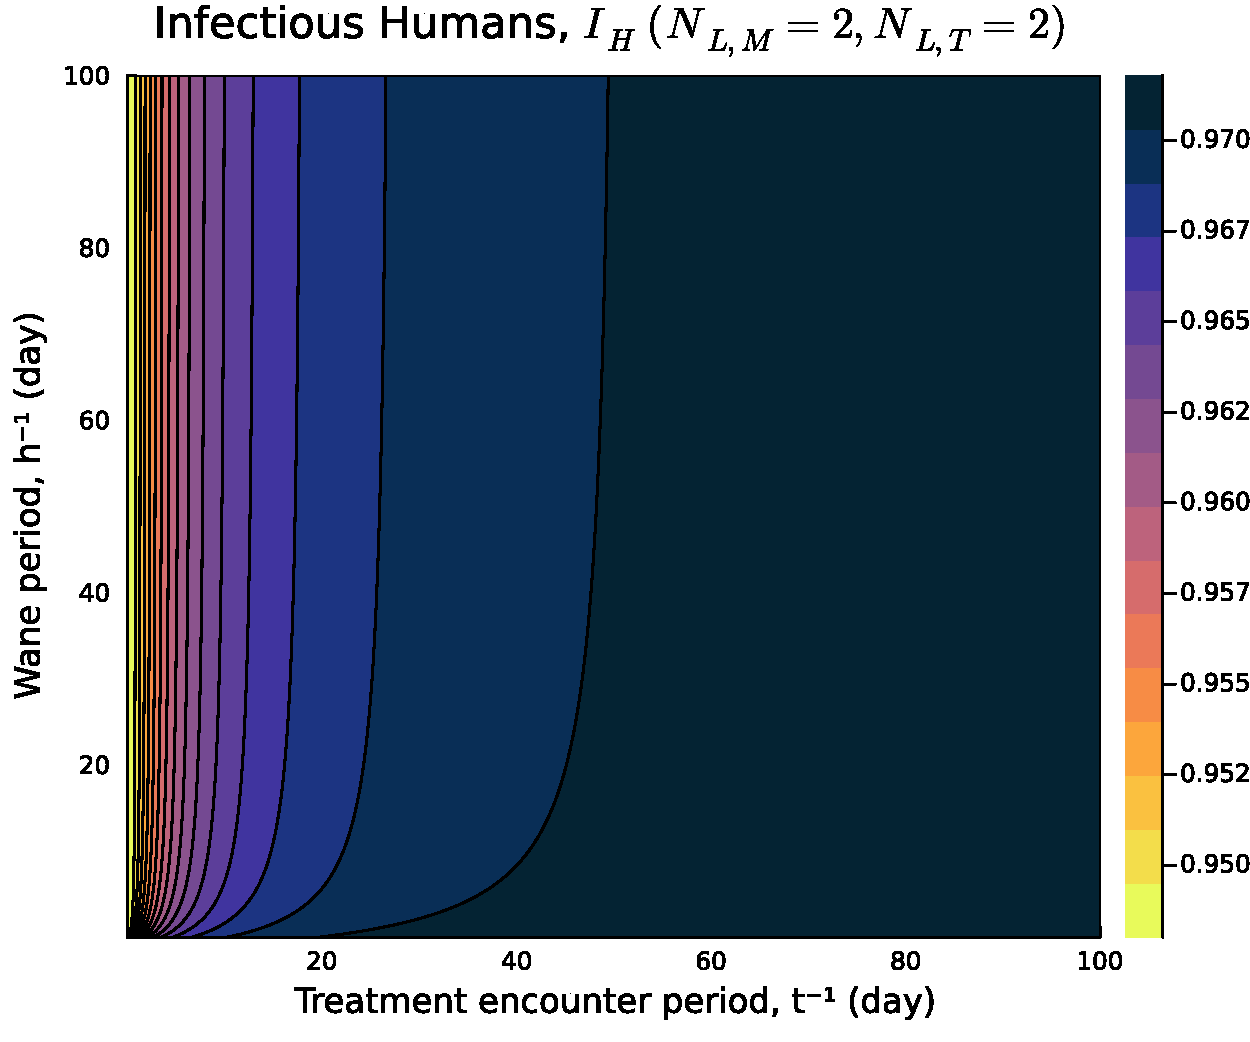
\includegraphics[width=0.4\textwidth]{../../fig/gen_model/IH_periods_txh_2x2.pdf}\\
    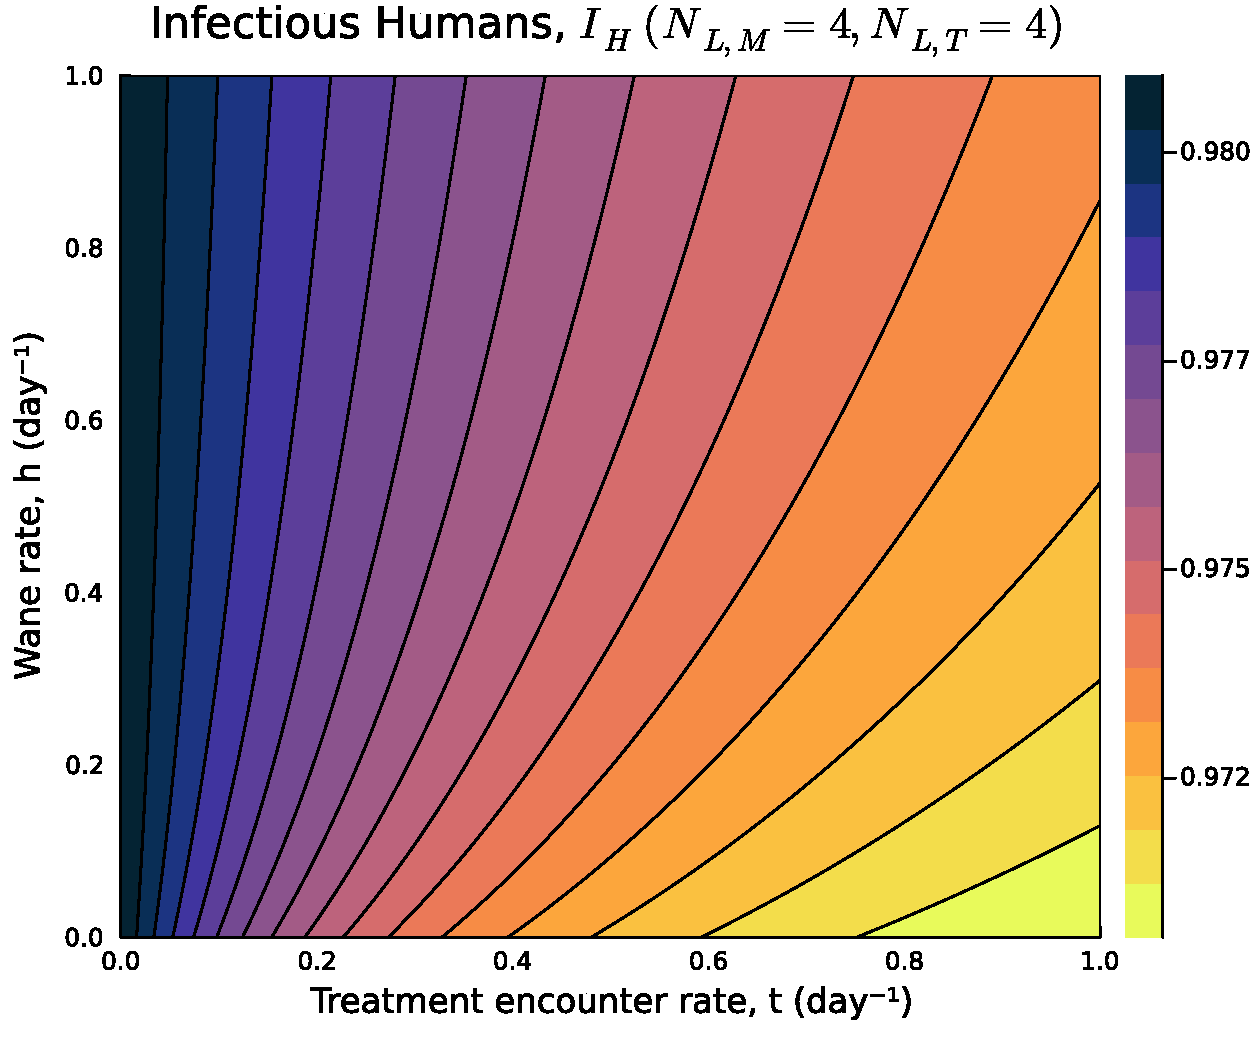
\includegraphics[width=0.4\textwidth]{../../fig/gen_model/IH_rates_txh_4x4.pdf}
    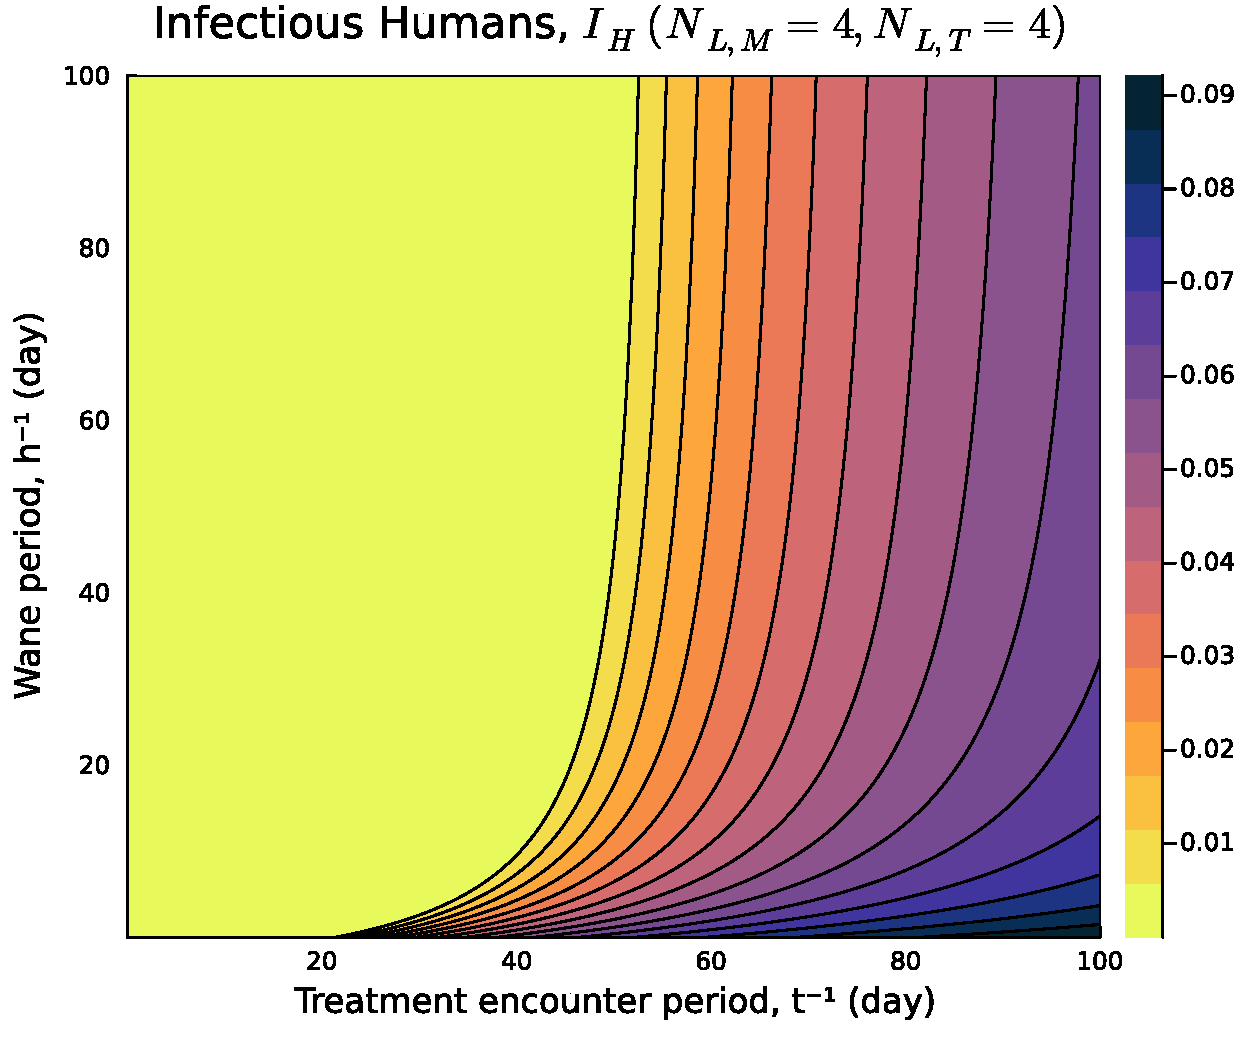
\includegraphics[width=0.4\textwidth]{../../fig/gen_model/IH_periods_txh_4x4.pdf}
    \caption{\textbf{Infections Humans at endemic equilibrium.} The left panels show the infected humans \(I_H\) as a function of the treatment rate, while the right panels show \(I_H\) as a function of the treatment period.}
\end{figure}

\begin{figure}[H]
    \centering
    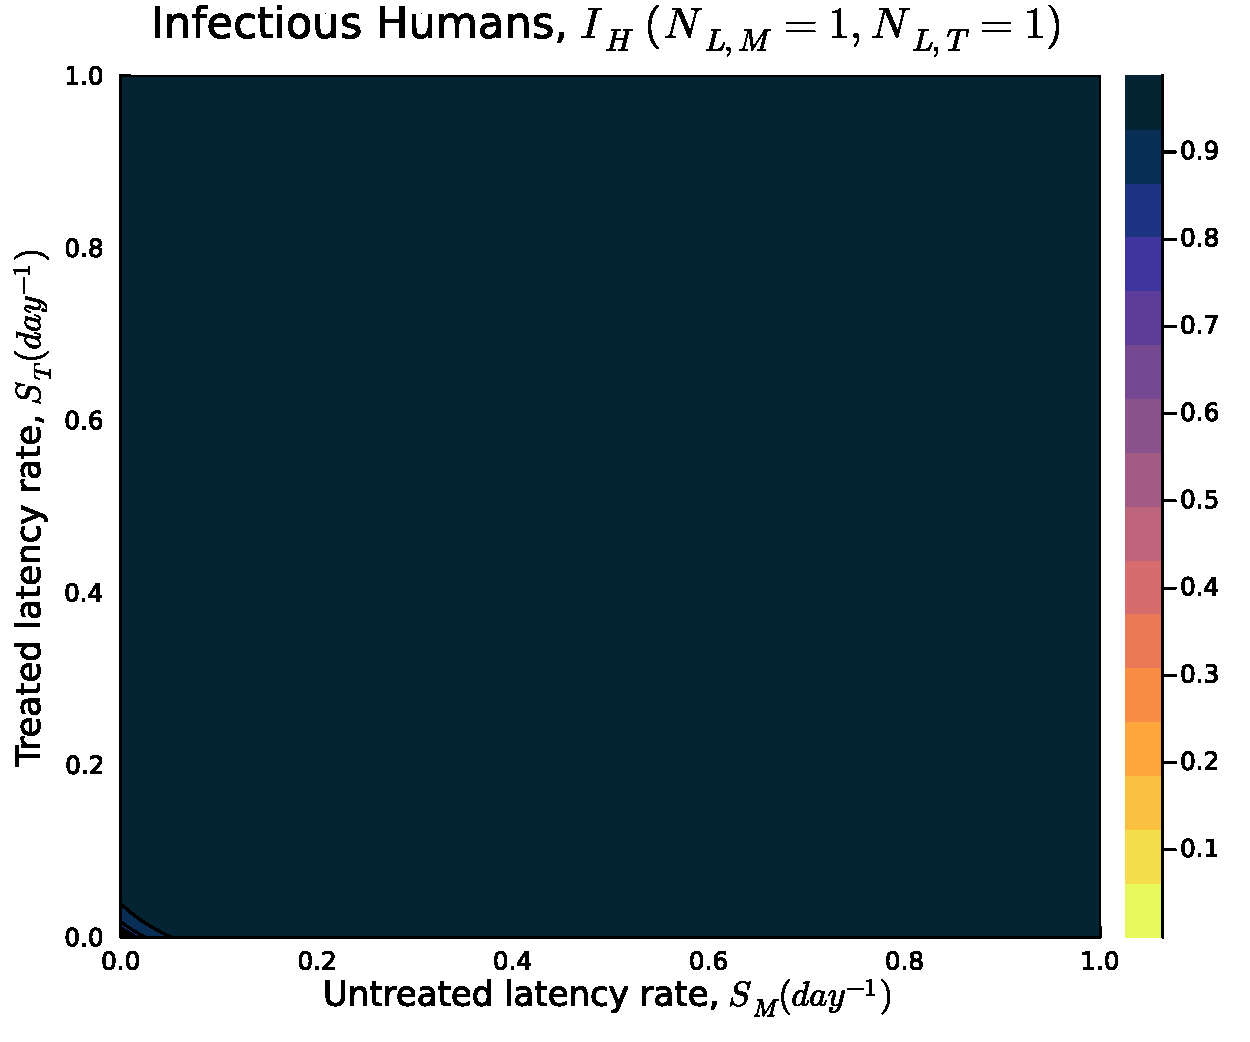
\includegraphics[width=0.4\textwidth]{../../fig/gen_model/IH_rates_SMxST_1x1.pdf}
    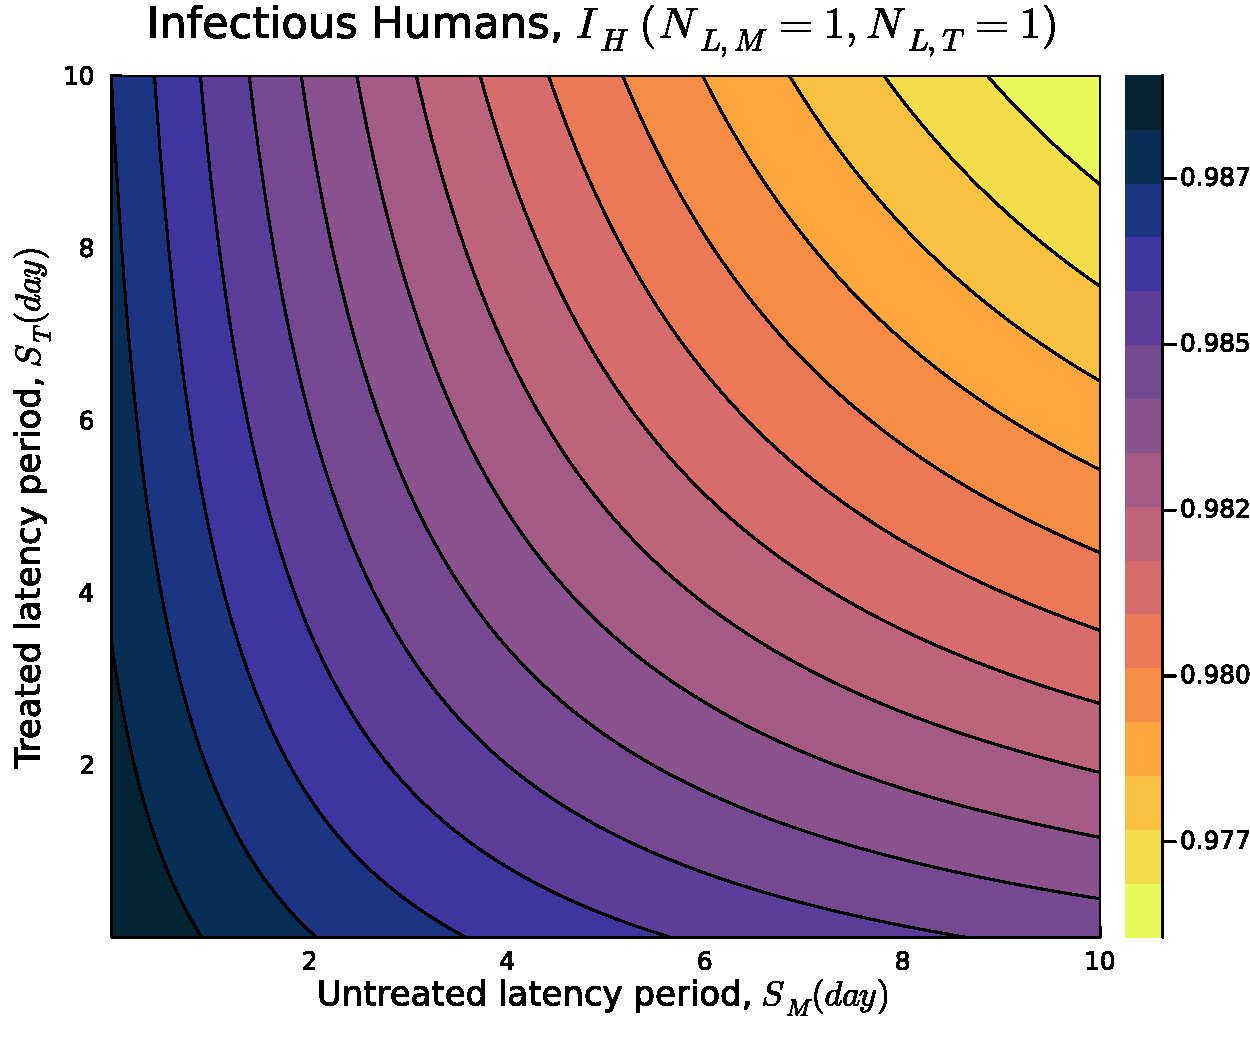
\includegraphics[width=0.4\textwidth]{../../fig/gen_model/IH_periods_SMxST_1x1.pdf}\\
    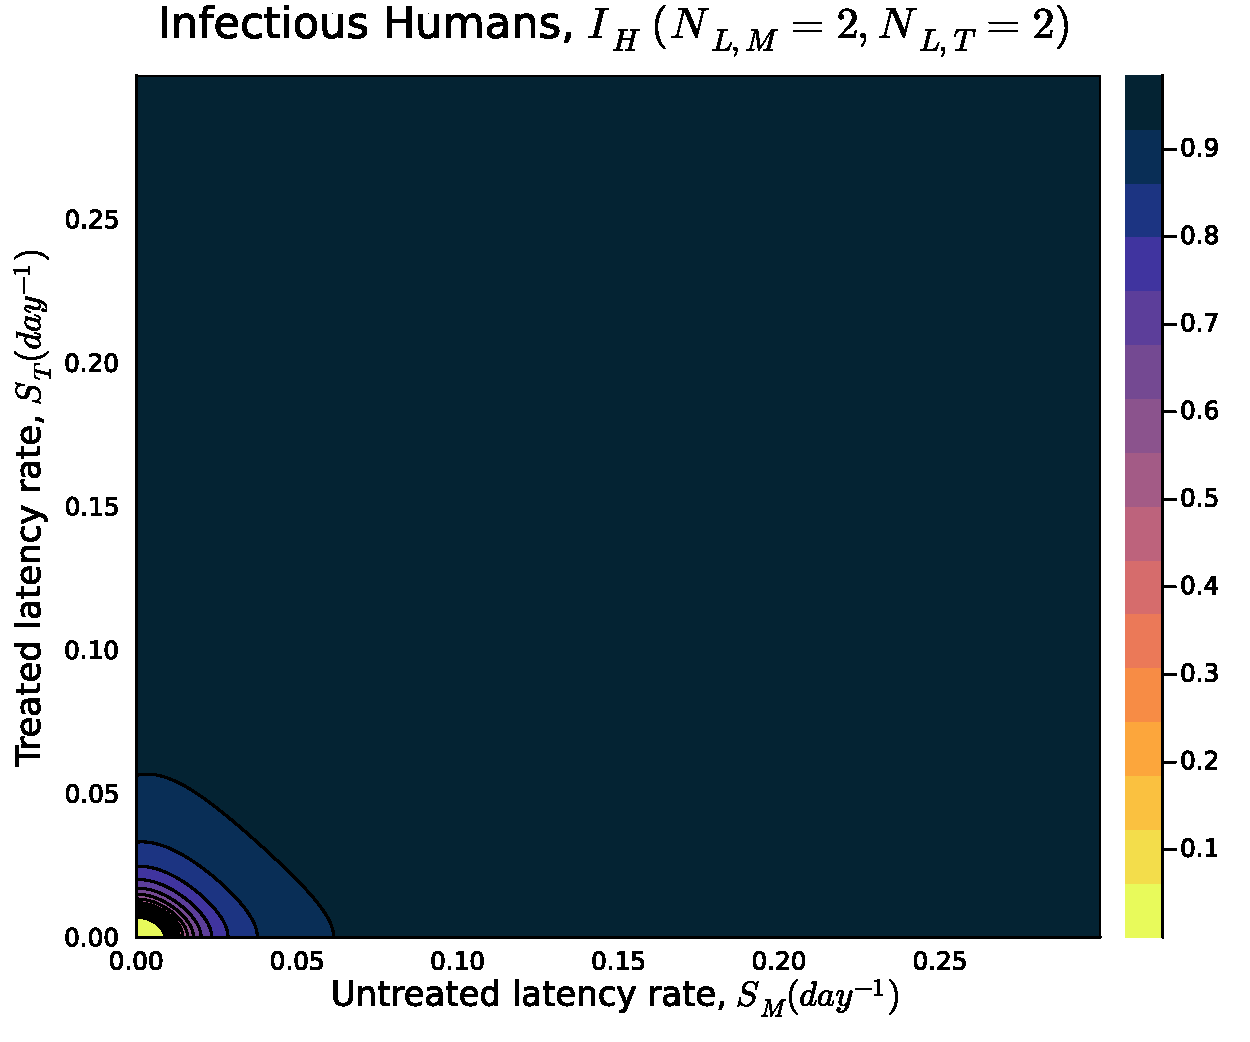
\includegraphics[width=0.4\textwidth]{../../fig/gen_model/IH_rates_SMxST_2x2.pdf}
    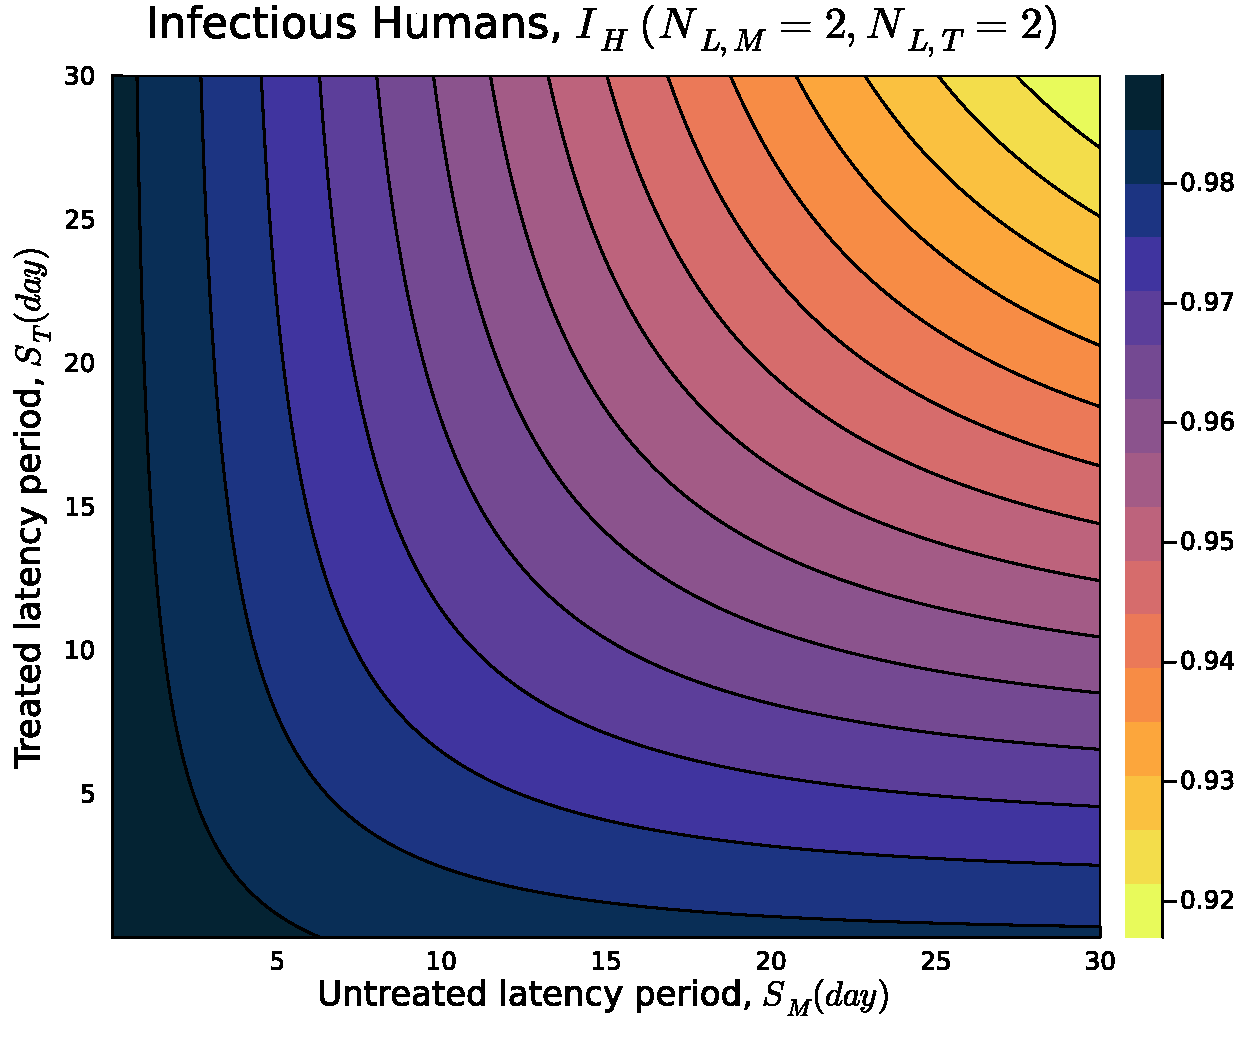
\includegraphics[width=0.4\textwidth]{../../fig/gen_model/IH_periods_SMxST_2x2.pdf}\\
    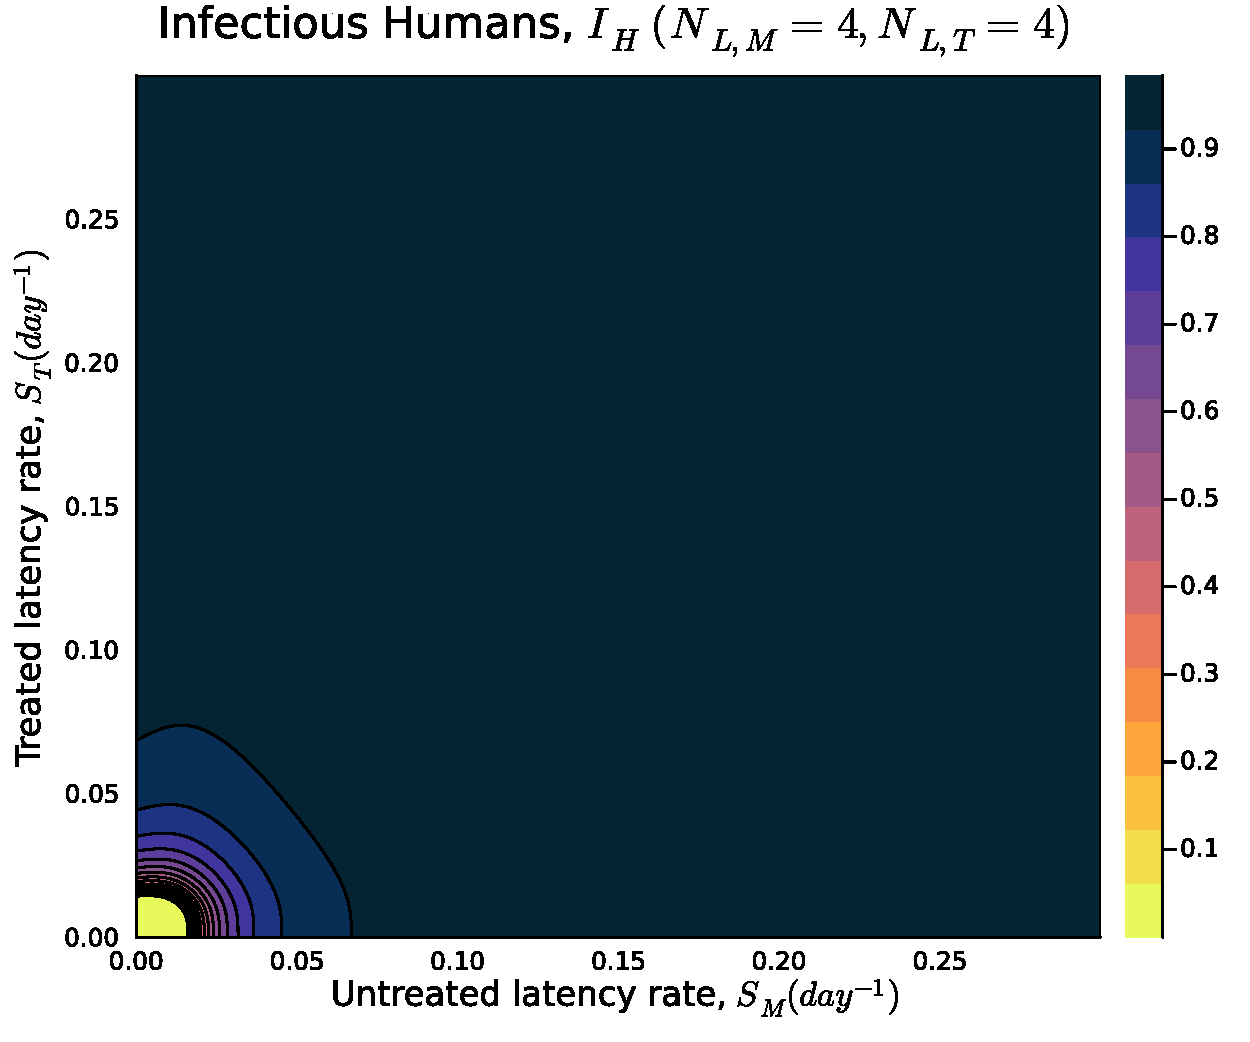
\includegraphics[width=0.4\textwidth]{../../fig/gen_model/IH_rates_SMxST_4x4.pdf}
    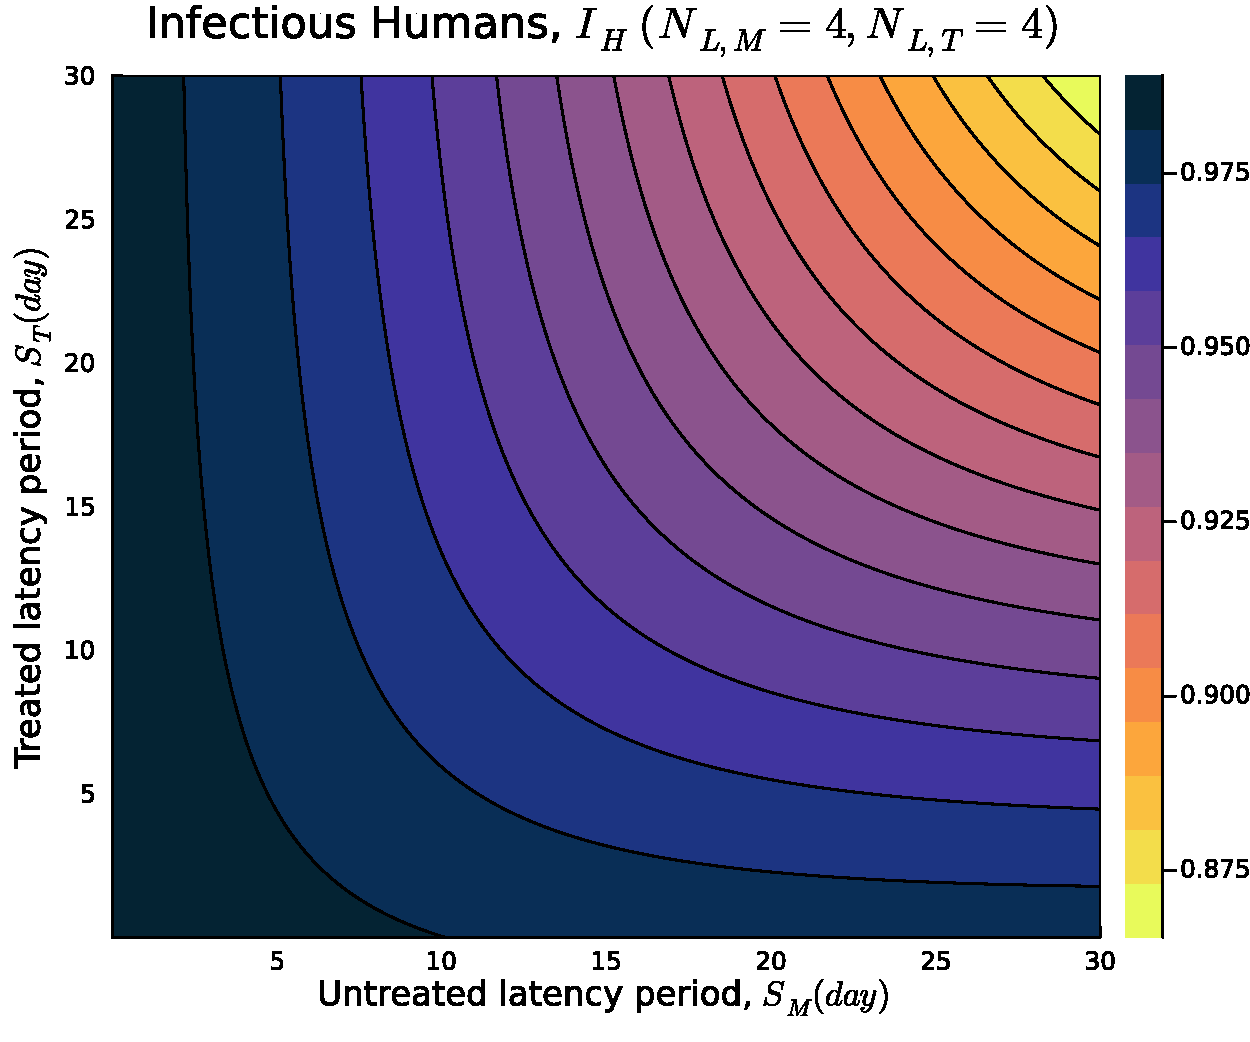
\includegraphics[width=0.4\textwidth]{../../fig/gen_model/IH_periods_SMxST_4x4.pdf}
    \caption{\textbf{Infections Humans at endemic equilibrium.} The left panels show the infected humans \(I_H\) as a function of the latency rate, while the right panels show \(I_H\) as a function of the latency period.}
\end{figure}

\end{document}
